% !TEX program = lualatex
%% Elsevier elsarticle + numbered references
\documentclass[5p,twocolumn]{elsarticle}

% \usepackage{luatexja}  % removed for English version
% \usepackage{luatexja-fontspec}  % removed for English version
\usepackage{amsmath,amssymb}
\usepackage{graphicx}
\usepackage{booktabs}
\usepackage{multirow}
\usepackage{siunitx}
\usepackage{xcolor}
\usepackage[colorlinks=true,linkcolor=blue,citecolor=blue,urlcolor=blue]{hyperref}
\usepackage{longtable}
\usepackage{array}
\usepackage{float}
\usepackage{enumitem}
\usepackage{subcaption}
\usepackage{listings}
\usepackage{algorithm}
\usepackage{algpseudocode}
\usepackage{tabularx}
\usepackage{url}
\usepackage{tikz}
\usetikzlibrary{arrows.meta,positioning,shapes.geometric,fit,calc,backgrounds}
\usepackage{lineno}
\biboptions{numbers}

\setlist{nosep,leftmargin=*}

% Japanese fonts (disabled for English version)
% \setmainjfont{IPAexMincho}
% \setsansjfont{IPAexGothic}

\lstset{
  basicstyle=\ttfamily\footnotesize,
  breaklines=true,
  frame=single,
  language=SQL,
  keywordstyle=\color{blue}\bfseries,
  commentstyle=\color{green!50!black},
  stringstyle=\color{red!70!black},
  numbers=left,
  numberstyle=\tiny\color{gray},
  tabsize=2,
}

\journal{---}

% =====================================================================
\begin{document}

\begin{frontmatter}

\title{Schema-Graph-Constrained Natural Language Interface for Intermetallic Compound Exploration}

\author[nims]{Satoshi Minamoto\corref{cor1}}
\cortext[cor1]{Corresponding author}
\ead{minamoto.satoshi@nims.go.jp}
\address[nims]{National Institute for Materials Science (NIMS),
  1-2-1 Sengen, Tsukuba, Ibaraki 305-0047, Japan}

\date{\today}

% =====================================================================
\begin{abstract}
Cross-sectional exploration of materials data accumulated in first-principles calculation databases
requires SQL expertise, posing a significant barrier for materials researchers.
This study proposes a Schema Graph-constrained Text-to-SQL method
that automatically generates SQL queries on normalized relational databases from natural-language questions.
The proposed method integrates a pipeline consisting of
foreign-key relationship representation as a graph with Steiner tree approximation for minimal JOIN path identification,
a domain-specific condition extractor for materials terminology normalization,
a multilayer SQL guard for table and column hallucination prevention,
and schema-constrained large language model (LLM) generation.
Using a validation database of 30 tables containing 1{,}470 entries centered on L1$_2$-type intermetallic compounds,
comparative experiments with five methods on 100 evaluation queries (up to 4-hop JOINs) showed that
the proposed method achieved a mean execution accuracy of 70.2\% with a syntax validity rate of 99\% and a table hallucination rate of 0\%,
representing an improvement of +43.6 percentage points over the full-schema baseline (26.6\%).
In an additional evaluation using 100 queries designed by an independent materials researcher,
an execution accuracy of 79.3\% was recorded while maintaining a syntax validity rate of 100\%.
For materials-engineering validation, the method achieved complete rediscovery of all 11 known L1$_2$ compounds
and ranking output of $\gamma'$ phase candidates.
Because the method is based on runtime introspection of foreign-key relationships,
it is applicable to arbitrary normalized materials databases.

\end{abstract}

\begin{keyword}
Text-to-SQL \sep L1$_2$-type intermetallic compounds \sep schema graph \sep Steiner tree approximation \sep $\gamma'$ phase \sep
materials database \sep natural language processing \sep materials informatics
\end{keyword}

\end{frontmatter}

% =====================================================================
\section{Introduction}
\label{sec:introduction}

\subsection{Data-Access Barriers in AI for Science and Materials Informatics}

The essential challenge of natural language interfaces for materials databases is
not the syntactic generation of SQL statements itself, but rather
correctly joining normalized heterogeneous materials data according to foreign-key relationships and materials-domain semantics.
In this paper, targeting the exploration of L1$_2$-type intermetallic compounds ($\gamma'$ phase candidates),
we propose a constrained method based on Schema Graph traversal
(a graph representation of FK relationships and Steiner tree approximation), and report that,
in an evaluation using 1{,}470 entries (5 prototypes) and 100 queries,
the Proposed method achieved a table hallucination rate of 0\% and an execution accuracy of 70.2\%.

\textbf{AI for Science (AI4S)}---the systematic application of artificial intelligence to accelerate scientific discovery---is
transforming materials research~\citep{wang2023ai4s,himanen2019dscribe}.
AI4S envisions integrated workflows in which AI agents autonomously generate hypotheses, retrieve relevant data from large-scale databases,
design experiments and simulations, and interpret results.
In this vision, \textbf{natural language access to structured materials data} is
not merely a convenience but a prerequisite:
if AI agents (or the researchers directing them) cannot efficiently query normalized relational databases,
the entire AI4S pipeline becomes bottlenecked at the data retrieval stage.

With the rapid development of high-throughput first-principles calculations,
multiple large-scale materials databases have been constructed:
the Open Quantum Materials Database (OQMD, approximately one million entries)~\citep{saal2013oqmd,kirklin2015oqmd},
Materials Project (over 150,000 entries)~\citep{jain2013mp},
AFLOW (over 3.5 million entries)~\citep{curtarolo2012aflow},
and NOMAD~\citep{draxl2019nomad}.
These databases are indispensable for computational materials exploration, screening of candidate phases~\citep{senkov2018hea,george2019hea},
and validation of experimental observations.
Meanwhile, as efforts toward structuring and knowledge representation of materials data,
Ishii et al. have constructed an ontology and RDF representation of the legacy superconductivity database SuperCon~\cite{ishii2023supercon} and
realized machine-readable conversion of the polymer database PoLyInfo~\cite{ishii2024polyinfo},
demonstrating that semantic structuring of schemas is a prerequisite for utilizing materials data.

However, access to data stored in normalized relational schemas
(multiple tables connected by foreign keys) requires SQL knowledge.
What is fundamentally important in materials engineering is not the collection of massive amounts of data but
\textbf{the accurate combination of small amounts of heterogeneous data}:
composition, crystal structure, thermodynamic stability, calculation conditions, and property values are
normalized into separate tables, and only by correctly JOINing them along foreign keys (FKs)
can meaningful materials information be obtained.
For example, retrieving ``lattice constants of stable B2 compounds containing Fe'' requires
a four-table JOIN with WHERE conditions on elements, prototypes, and thermodynamic stability---an easy task for a database engineer, but
a nontrivial operation for a materials researcher.
Inaccurate JOINs (unnecessary table joins or missing join conditions)
return erroneous combinations of data and pose a serious risk of misleading decisions in materials exploration and screening.

REST APIs and GraphQL endpoints provided by many materials databases
partially alleviate this barrier, but fundamental constraints common to RDBs remain:
(a)~dependence on predefined filter syntax (making ad hoc compound conditions and aggregation difficult),
(b)~risk of API incompatibility when schemas are updated, and
(c)~the frequent absence of APIs for in-house databases or independently extended schemas.
Because the T2SQL approach analyzes schema structures at runtime,
it is in principle applicable to arbitrary normalized RDBs regardless of the presence or absence of an API
(although preparation of terminology dictionaries and performance validation for large-scale schemas are separately required).

In the context of AI4S, this data-access barrier is particularly serious:
autonomous AI agents performing materials screening or property prediction
must programmatically issue complex compound-condition database queries.
A natural language interface that reliably generates correct SQL
enables both human researchers and AI agents to interact with materials databases without expertise in database engineering,
thereby removing a key bottleneck in AI4S workflows.

\subsection{Technical Trends in Text-to-SQL}

Text-to-SQL (T2SQL) research has advanced rapidly through large-scale benchmarks:
Spider~\citep{yu2018spider} (10,181 questions, 200 databases, 138 domains) and
BIRD~\citep{li2024bird} (12,751 questions, 95 databases, 33.4~GB).
Recent LLM-based methods have achieved high accuracy:
DAIL-SQL~\citep{gao2023dail} reported an execution accuracy of 86.6\% on Spider through skeleton-based few-shot example selection,
DIN-SQL~\citep{pourreza2024dinsql} achieved 85.3\% through decomposed in-context learning, and
XiYan-SQL~\citep{gao2024xiyan} reported further accuracy improvements using a multi-generator ensemble.
Hong et al.~\citep{hong2024survey} provide a comprehensive survey highlighting the dominant role of schema linking,
and Maamari et al.~\citep{maamari2024schema} argue that explicit schema linking may become unnecessary with advanced LLMs,
although this remains under debate.

Methods that explicitly use schema structures as graphs have also developed.
RAT-SQL~\citep{wang2020ratsql} pretrains inter-table relationships through Relation-Aware Schema Encoding, and
ShadowGNN~\citep{chen2021shadowgnn} encodes schema graphs using a graph projection neural network.
RESDSQL~\citep{li2023resdsql} separates schema linking and skeleton parsing, and
Bridge~\citep{lin2020bridge} bridges text and tabular data.
More recently, SchemaGraphSQL~\citep{safdarian2026schemagraphsql} proposed large-scale database schema linking using path-finding algorithms, and
GraST-SQL~\citep{hoang2025grastsql} addresses scaling of schema filtering using functional dependency graphs.
McMillan~\citep{mcmillan2026context} evaluates the impact of structured context engineering on
schema accuracy in multi-file agent systems.

However, \textbf{all existing T2SQL benchmarks target general-purpose domains}
(e-commerce, healthcare, and education), and no prior study has addressed
challenges specific to materials science databases:
domain-specific terminology (Strukturbericht symbols and prototype names),
bilingual queries (Japanese and English element names),
normalization of composition tables (one row per element per compound), and
thermodynamic stability filters ($E_\text{hull} \leq 0.001$~eV/atom).

\subsection{NLP in Materials Informatics}

Applications of NLP in materials science are expanding:
MatSci-NLP~\citep{song2023matscnlp} benchmarks seven NLP tasks for materials texts,
LLAMAT~\citep{mishra2024llamat} improves information extraction through continued pretraining of LLaMA,
the Materials Knowledge Navigation Agent (MKNA)~\citep{zhuang2026mkna} converts
natural language intents into database search and structure-generation actions, and
OptiMat Alloys~\citep{hu2026optimat} provides an LLM-driven interactive alloy exploration tool.
Materials Project has begun providing MCP-based LLM integration~\citep{mp_mcp2025}.

Although these studies address information extraction and agent-based database interaction,
none targets \textbf{schema-aware SQL generation over normalized relational databases}---in particular,
automatic JOIN path discovery through foreign-key graph traversal.
This gap is the focus of the present method.

\subsection{Relationship to Ontology and Knowledge Graph Approaches}
\label{sec:ontology_comparison}

For structured access to materials data,
approaches based on ontologies and knowledge graphs (KGs) also constitute a prominent lineage.
Ishii et al. reconstructed the superconducting materials database SuperCon as an RDF ontology and
realized semantic search through a SPARQL endpoint~\citep{ishii2023supercon}.
The same group also performed similar machine-readable conversion for polymer data in PoLyInfo,
enabling cross-domain data integration through alignment with the BFO upper ontology~\citep{ishii2024polyinfo}.
In Europe, the Elementary Multiperspective Material Ontology (EMMO) has been developed
as a standard ontology for materials modeling,
providing guarantees of semantic consistency based on OWL reasoning~\citep{emmo2020}.

In general-purpose domains, Sequeda \& Allemang~\citep{sequeda2024benchmark} converted
enterprise SQL databases into knowledge graphs and showed that
Text-to-SPARQL improves accuracy from 16\% to 54\% compared with Text-to-SQL.
Furthermore, query validation using ontology semantic constraints (OBQC) improved accuracy to
72\%~\citep{allemang2024obqc}.

The present method shares with these ontology approaches the objective of
\textbf{query quality assurance through structural constraints}.
Domain/range constraints in OWL properties of ontologies functionally correspond to
inter-table constraints imposed by FK relationships in RDBs, and
SPARQL query validation by OBQC plays a role equivalent to that of
SQLGuard in the present method (column whitelisting and FK-consistent JOIN validation).
However, the application contexts of the two approaches differ.
Ontology approaches presuppose data conversion into RDF triple stores and
have superior expressive power for semantic transitivity through OWL reasoning
(e.g., ``NiAl is L1$_2$-type'' $\to$ ``NiAl is an intermetallic compound'') and
interoperability among heterogeneous databases.
In contrast, large-scale materials databases such as OQMD~\citep{saal2013oqmd}, Materials Project~\citep{jain2013mp}, and AFLOW~\citep{curtarolo2012aflow}
are already operated using relational schemas, and
the present method adopts a design that \textbf{leverages these existing RDB infrastructures as they are}.
Graph traversal of FK relationships (Steiner tree approximation) provides
a lightweight alternative that guarantees the correctness of JOIN paths without relying on ontology reasoning.

The two approaches are not mutually exclusive but complementary.
In the future, integrating semantic constraints defined by ontologies into
Schema Graph traversal heuristics may enable JOIN path selection based not only on FK relationships
but also on domain knowledge.

\subsection{Objectives and Novelty}

The contributions of this study are the following five points:

\begin{enumerate}
  \item \textbf{A Schema Graph-constrained T2SQL method specialized for L1$_2$-type compound exploration}:
    by combining a Japanese--English bilingual materials terminology dictionary with FK relationship graph traversal,
    the method realizes automatic JOIN path computation on normalized materials databases,
    including synonym normalization for expressions such as L1$_2$/$\gamma'$/Cu$_3$Au-type.
    Schema Graph constraints achieve a \textbf{table hallucination rate of 0\%},
    eliminating hallucinations in the LLM-only method while
    achieving an \textbf{execution accuracy of 70.2\%} by eliminating unnecessary JOINs.
  \item \textbf{Quantitative evaluation through comparison with five method baselines}:
    five methods---LLM-only, Full Schema, Rule-based, FK-list, and Proposed---are compared using
    100 queries (Easy/Medium/Hard/Very Hard, up to 4-hop),
    systematically evaluating the effect of how schema information is presented on SQL quality.
  \item \textbf{Safety assurance through a multilayer SQL guard}:
    keyword blacklisting, table/column whitelisting,
    JOIN validation, and automatic LIMIT injection are integrated to
    prevent execution of invalid SQL.
  \item \textbf{Materials-engineering evaluation}:
    the method achieves complete rediscovery (11/11) of the 11 known L1$_2$ compounds,
    ranking of $\gamma'$ phase candidates, extraction of candidates with lattice constants near that of Ni$_3$Al,
    and automatic generation of materials-design hypotheses.
  \item \textbf{Multihop query evaluation}:
    for 47 multihop queries requiring 2--4 table JOINs,
    we report the execution accuracy of the Proposed method and comparisons with each baseline.
\end{enumerate}

The overall architecture of the present method is shown in Fig.~\ref{fig:step3_pipeline} (overview) and
Fig.~\ref{fig:architecture} (detailed configuration).

% --- Step 3 pipeline figure (corresponding to Step 3 in HTML) ---
\begin{figure*}[htbp]
\centering
\resizebox{\textwidth}{!}{%
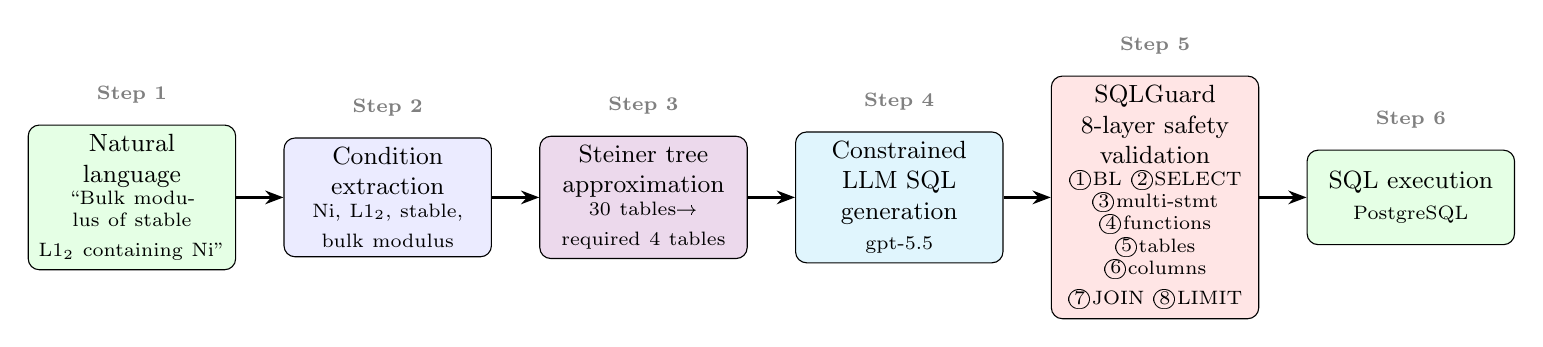
\begin{tikzpicture}[
  node distance=0.3cm and 0.6cm,
  >=Stealth,
  every node/.style={font=\small},
  stepbox/.style={rectangle, draw, rounded corners=4pt,
    minimum height=1.2cm, minimum width=2.2cm, align=center,
    text width=2.4cm},
  arr/.style={->, thick, >=Stealth},
]

% Step boxes
\node[stepbox, fill=green!10] (nl) {Natural language\\
  {\scriptsize ``Bulk modulus of stable\\ L1$_2$ containing Ni''}};

\node[stepbox, fill=blue!8, right=of nl] (extract) {Condition extraction\\
  {\scriptsize Ni, L1$_2$, stable,\\ bulk modulus}};

\node[stepbox, fill=violet!15, right=of extract] (steiner) {Steiner tree approximation\\
  {\scriptsize 30 tables→\\ required 4 tables}};

\node[stepbox, fill=cyan!12, right=of steiner] (llmgen) {Constrained\\ LLM SQL generation\\
  {\scriptsize gpt-5.5}};

\node[stepbox, fill=red!10, right=of llmgen] (guard) {SQLGuard\\ 8-layer safety validation\\
  {\scriptsize \textcircled{\scriptsize 1}BL
  \textcircled{\scriptsize 2}SELECT
  \textcircled{\scriptsize 3}multi-stmt\\
  \textcircled{\scriptsize 4}functions
  \textcircled{\scriptsize 5}tables
  \textcircled{\scriptsize 6}columns\\
  \textcircled{\scriptsize 7}JOIN
  \textcircled{\scriptsize 8}LIMIT}};

\node[stepbox, fill=green!10, right=of guard] (exec) {SQL execution\\
  {\scriptsize PostgreSQL}};

% Arrows
\draw[arr] (nl) -- (extract);
\draw[arr] (extract) -- (steiner);
\draw[arr] (steiner) -- (llmgen);
\draw[arr] (llmgen) -- (guard);
\draw[arr] (guard) -- (exec);

% Step labels
\node[above=0.15cm of nl, font=\scriptsize\bfseries, color=gray] {Step 1};
\node[above=0.15cm of extract, font=\scriptsize\bfseries, color=gray] {Step 2};
\node[above=0.15cm of steiner, font=\scriptsize\bfseries, color=gray] {Step 3};
\node[above=0.15cm of llmgen, font=\scriptsize\bfseries, color=gray] {Step 4};
\node[above=0.15cm of guard, font=\scriptsize\bfseries, color=gray] {Step 5};
\node[above=0.15cm of exec, font=\scriptsize\bfseries, color=gray] {Step 6};

\end{tikzpicture}%
}% end resizebox
\caption{Overview of the Step 3 pipeline.
  Starting from a natural language query and condition extraction (Step 2),
  Steiner tree approximation (Step 3) extracts the minimal necessary subgraph from 30 tables.
  The extracted tables, columns, and JOIN conditions are injected into the LLM as YAML (Step 4),
  and safe SQLFN is executed after passing through the 8-layer SQLGuard (Step 5).
  Because the LLM's field of view is limited to the necessary tables,
  unnecessary JOINs and table hallucinations are eliminated in principle.}
\label{fig:step3_pipeline}
\end{figure*}
% =====================================================================
\section{Design Requirements for Materials Text-to-SQL}
\label{sec:design_requirements}

The essential challenge of a natural-language interface for materials databases is
not the syntactic generation of SQL statements itself,
but rather
\textbf{correctly joining normalized heterogeneous materials data according to foreign-key relationships and materials-domain semantics}.
When a general-purpose Text-to-SQL system is directly applied to a materials database,
the following materials-specific requirements are not satisfied, leading to a substantial degradation in accuracy.

\begin{enumerate}
  \item \textbf{Accurate JOINs of normalized composition tables}:
    Because each element in a multicomponent compound is stored as an independent row,
    searches for compounds containing \emph{both} ``Ni and Al'' require a SELF-JOIN or INTERSECT.
    General-purpose LLMs frequently make errors in this pattern.
  \item \textbf{Disambiguation of materials terminology}:
    Whether ``NiAl'' denotes a specific compound (B2-NiAl) or a contained-element condition is context-dependent,
    and whether ``stable'' means $E_\mathrm{hull} \leq 0.001$~eV/atom or
    $\Delta G_f < 0$ is schema-dependent.
    Without a domain dictionary, column mapping becomes indeterminate.
  \item \textbf{Vocabulary normalization of prototypes and space groups}:
    L1$_2$, AuCu$_3$ type, and Cu$_3$Au type refer to the same prototype,
    but their notations are diverse, requiring synonym expansion in both Japanese and English.
  \item \textbf{Computation of minimal JOIN paths along FKs}:
    In a schema with approximately 30 tables, candidate JOIN paths proliferate,
    and joining unnecessary tables reduces LLM accuracy.
    Extracting a minimal subgraph via a Steiner tree approximation is indispensable.
  \item \textbf{Interpretation of units and thresholds in numerical conditions}:
    Whether ``a large band gap'' means $> 1.0$~eV or $> 2.0$~eV,
    and whether ``stable'' means $E_\mathrm{hull} \leq 0.001$ or $\leq 0.1$
    requires judgment based on materials-domain knowledge.
  \item \textbf{Rejection of out-of-scope questions}:
    Questions about the optimization of VASP calculation parameters or DFT workflows are
    not SQL-answerable, and forcing SQL generation returns meaningless results.
  \item \textbf{Guarantees for safe execution}:
    Exclusion of non-SELECT SQL (INSERT/UPDATE/DELETE),
    prevention of unrestricted result sets (automatic LIMIT injection),
    and injection prevention using table and column whitelists.
\end{enumerate}

These requirements are materials-database-specific challenges that are
not included as evaluation targets in general-purpose Text-to-SQL benchmarks (Spider, WikiSQL, etc.).
The proposed method was designed as an integrated framework that addresses all seven requirements above.
% =====================================================================
\section{Methods}
\label{sec:methods}

This section details each technical component.
Figure~\ref{fig:architecture} shows the overall pipeline architecture of the system.

\begin{figure*}[htbp]
\centering
\resizebox{\textwidth}{!}{%
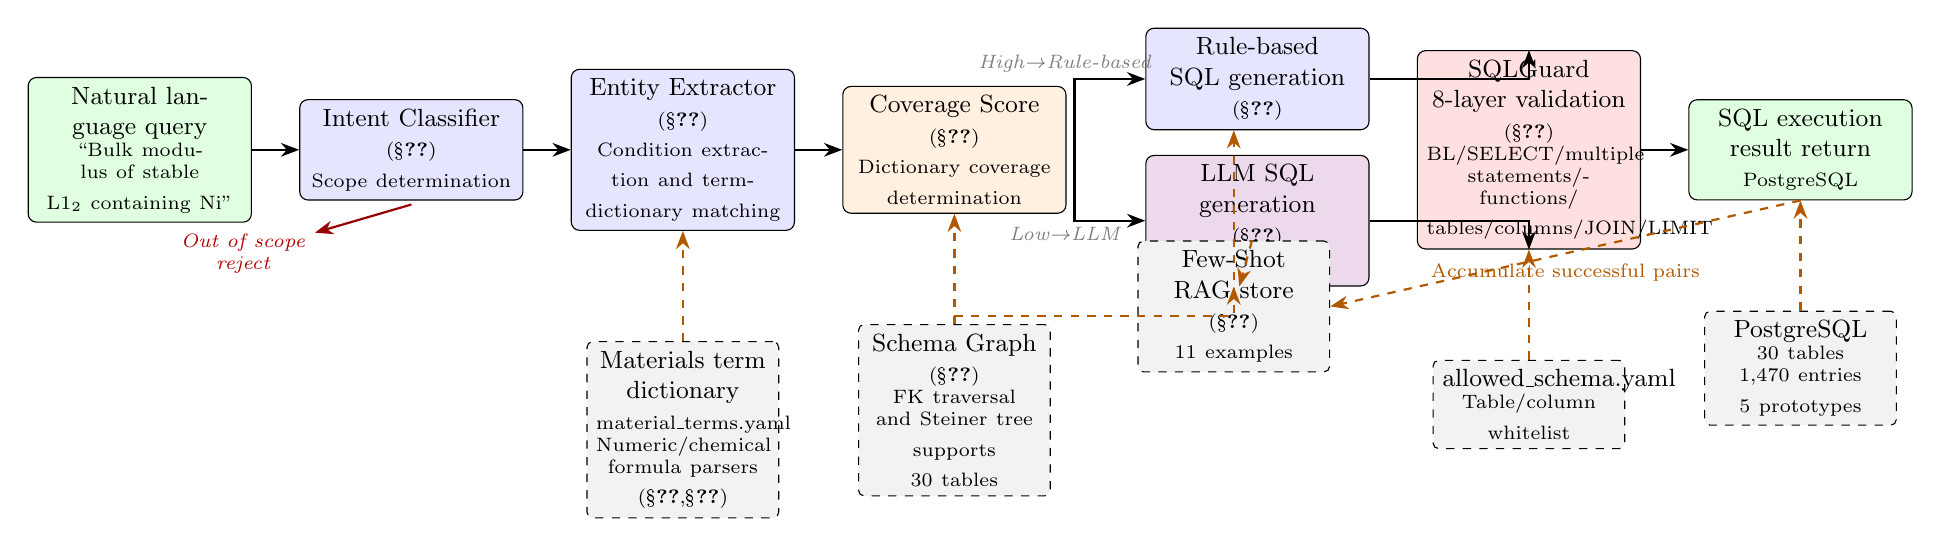
\begin{tikzpicture}[
  node distance=0.4cm and 0.5cm,
  >=Stealth,
  every node/.style={font=\small},
  module/.style={rectangle, draw, rounded corners=3pt,
    minimum height=1.0cm, minimum width=2.4cm, align=center,
    text width=2.6cm},
  store/.style={rectangle, draw, dashed, rounded corners=2pt,
    minimum height=0.8cm, align=center,
    fill=gray!10, text width=2.2cm},
  arr/.style={->, thick, >=Stealth},
  darr/.style={->, thick, dashed, >=Stealth, color=orange!70!black},
  lbl/.style={font=\scriptsize, midway},
]

% === Layer 1: Input ===
\node[module, fill=green!12] (input) {Natural language query\\{\scriptsize “Bulk modulus of stable\\ L1$_2$ containing Ni”}};

% === Layer 2: Intent & Extraction ===
\node[module, fill=blue!10, right=0.6cm of input] (intent) {Intent Classifier\\{\scriptsize (\S\ref{sec:intent_classifier})}\\{\scriptsize Scope determination}};

\node[module, fill=blue!10, right=0.6cm of intent] (extract) {Entity Extractor\\{\scriptsize (\S\ref{sec:entity_extractor})}\\{\scriptsize Condition extraction and term-dictionary matching}};

% === Layer 3: Coverage → Branching ===
\node[module, fill=orange!12, right=0.6cm of extract] (coverage) {Coverage Score\\{\scriptsize (\S\ref{sec:coverage_score})}\\{\scriptsize Dictionary coverage determination}};

% === Layer 4: Dual Generation ===
\node[module, fill=blue!10, right=1.0cm of coverage, yshift=0.9cm] (rb) {Rule-based\\SQL generation\\{\scriptsize (\S\ref{sec:sql_generation})}};
\node[module, fill=violet!15, right=1.0cm of coverage, yshift=-0.9cm] (llm) {LLM SQL generation\\{\scriptsize (\S\ref{sec:llm_mode})}\\{\scriptsize gpt-5.5}};

% === Layer 5: Guard ===
\node[module, fill=red!12, right=0.6cm of rb, yshift=-0.9cm] (guard) {SQLGuard\\8-layer validation\\{\scriptsize (\S\ref{sec:sql_guard})}\\{\scriptsize BL/SELECT/multiple statements/functions/\\tables/columns/JOIN/LIMIT}};

% === Layer 6: Output ===
\node[module, fill=green!12, right=0.6cm of guard] (exec) {SQL execution\\result return\\{\scriptsize PostgreSQL}};

% === Data Stores (bottom) ===
\node[store, below=1.4cm of extract] (dict) {Materials term dictionary\\{\scriptsize material\_terms.yaml}\\{\scriptsize Numeric/chemical formula parsers\\(\S\ref{sec:numeric_parser},\S\ref{sec:formula_parser})}};

\node[store, below=1.4cm of coverage] (sg) {Schema Graph\\{\scriptsize (\S\ref{sec:schema_graph})}\\{\scriptsize FK traversal and Steiner tree\\supports 30 tables}};

\node[store, below=1.4cm of rb, xshift=-0.3cm] (rag) {Few-Shot RAG store\\{\scriptsize (\S\ref{sec:few_shot})}\\{\scriptsize 11 examples}};

\node[store, below=1.4cm of guard] (yaml) {allowed\_schema.yaml\\{\scriptsize Table/column\\whitelist}};

\node[store, below=1.4cm of exec] (db) {PostgreSQL\\{\scriptsize 30 tables\\1{,}470 entries\\5 prototypes}};

% === Arrows: Main flow ===
\draw[arr] (input) -- (intent);
\draw[arr] (intent) -- (extract);
\draw[arr] (extract) -- (coverage);
\draw[arr] (coverage.east) ++(0.1,0) |- (rb.west);
\draw[arr] (coverage.east) ++(0.1,0) |- (llm.west);
\draw[arr] (rb.east) -| (guard.north);
\draw[arr] (llm.east) -| (guard.south);
\draw[arr] (guard) -- (exec);

% === Arrows: Data stores ===
\draw[darr] (dict) -- (extract);
\draw[darr] (sg) -- (coverage);
\draw[darr] (sg.north) ++(0,0.1) -| ([xshift=-0.3cm]rb.south);
\draw[darr] (sg.north) ++(0,0.1) -| ([xshift=-0.3cm]llm.south);
\draw[darr] (rag) -- (llm);
\draw[darr] (yaml) -- (guard);
\draw[darr] (db) -- (exec);

% === Labels ===
\node[above=0.05cm of coverage, font=\scriptsize\itshape, xshift=1.4cm, color=gray] {High→Rule-based};
\node[below=0.05cm of coverage, font=\scriptsize\itshape, xshift=1.4cm, color=gray] {Low→LLM};

% === Feedback loop ===
\draw[darr, bend left=15] (exec.south) -- node[below, font=\scriptsize, color=orange!70!black] {Accumulate successful pairs} (rag.east);

% === Reject ===
\node[below left=0.3cm and -0.2cm of intent, font=\scriptsize\itshape, text=red!70!black, align=center] (reject) {Out of scope\\reject};
\draw[arr, red!60!black] (intent.south) ++(0,-0.05) -- (reject);

\end{tikzpicture}%
}% end resizebox
\caption{Overall configuration of the system architecture.
  Solid arrows indicate the main data flow, and dashed arrows (orange) indicate data references and feedback loops.
  Based on the Coverage Score, the pipeline branches to either the Rule-based path (high coverage) or the LLM path (low coverage),
  and in both cases, safe SQL is generated and executed through JOIN-path constraints imposed by the
  Schema Graph (FK traversal over 30 tables) and
  SQLGuard 8-layer validation.
  When an execution error or an empty result is detected,
  a repair loop (up to 2 attempts) is activated, requesting the LLM to perform a repair with error diagnostic information.
  Successful query pairs are accumulated in the Few-Shot RAG store and used for subsequent LLM generation.}
\label{fig:architecture}
\end{figure*}

\subsection{Database Schema Design for Materials Data}
\label{sec:schema_design}

\subsubsection{Normalized Schema Design for OQMD Data}

OQMD systematically stores composition, structure, and thermodynamic stability,
and is a representative example of the schema complexity typical of materials databases
(many-to-many relationships, normalized composition tables,
and separation of structural parameters).
Flat JSON records obtained from the API are normalized into a relational schema
(Table~\ref{tab:schema}).
The design follows Boyce-Codd normal form (BCNF) and is based on the following materials-domain-specific considerations.



\begin{table*}[htbp]
  \centering
  \caption{Overview of the database schema.}
  \label{tab:schema}
  \small
  \begin{tabularx}{\textwidth}{lllX}
    \toprule
    Table name & Primary key & Foreign key & Main columns \\
    \midrule
    material\_entry & entry\_id & --- & formula, reduced\_formula, chemical\_system \\
    composition & composition\_id & entry\_id & element, atomic\_fraction \\
    structure & structure\_id & entry\_id & prototype, strukturbericht, lattice\_a, space\_group \\
    phase\_stability & stability\_id & entry\_id & formation\_energy\_per\_atom, energy\_above\_hull, band\_gap \\
    calculation & calculation\_id & entry\_id & method, functional \\
    calculated\_property & property\_id & calculation\_id & property\_name, value, unit \\
    prototype\_definition & prototype\_id & --- & prototype\_name, strukturbericht, description \\
    \bottomrule
  \end{tabularx}
\end{table*}

\paragraph{Separation of the Composition Table}
A single compound may contain multiple elements (e.g., Fe$_3$Al $\to$ Fe and Al).
By storing each element as a separate row in the \texttt{composition} table,
flexible element-based queries (AND, OR, NOT) are enabled without string parsing~\citep{villars2004pauling}.
However, this normalization introduces an important complexity:
a query for “compounds containing both Ni and Al” cannot be expressed by a simple
\texttt{WHERE element = 'Ni' AND element = 'Al'}
(because no single row can satisfy both conditions simultaneously, 0 rows are returned).
Instead, \texttt{EXISTS} subqueries are required (see Section~\ref{sec:multi_element}).
This design also enables searches that do not depend on the notation order of chemical formulas
(e.g., Ni$_3$Al and AlNi$_3$ are the same compound, but notation conventions differ across
databases).
Because elements and atomic fractions are stored as separate rows, the same compound can be uniquely identified
by element-level queries rather than by string comparison of the entire formula.

\paragraph{Separation of Structure/Phase Stability/Calculation}
Crystal structure information (prototype, lattice constants), thermodynamic stability (energy above hull),
and calculation metadata (DFT functional) are stored in separate tables,
enabling independent updates and extensions.

\paragraph{Entity-Attribute-Value (EAV) Pattern for Calculated Properties}
The \texttt{calculated\_property} table uses the EAV pattern
(\texttt{property\_name}, \texttt{value}, \texttt{unit}),
allowing arbitrary calculated properties (bulk modulus, shear modulus, etc.) to be accommodated without schema changes.
In the EAV design, in addition to the column whitelist,
a list of permitted values for \texttt{property\_name} (\texttt{bulk\_modulus}, \texttt{shear\_modulus}, etc.)
is maintained, enabling detection when the LLM generates a nonexistent property name.

\paragraph{Note on the Generality of ER Design}
Although OQMD is internally operated on a relational database (Django ORM + PostgreSQL),
in this study we newly designed an ER diagram that is easy to traverse as a
NetworkX graph and YAML schema, using the flat JSON data obtained from the API.
This design decision generalizes the applicability of the proposed method to the following two scenarios:
(1)~directly extracting and traversing schema information (FK constraints) from an existing RDB,
and (2)~constructing and traversing a new purpose-specific ER diagram from flat data.
In either case, if FK relationships can be represented as a graph,
JOIN-path optimization by Schema Graph traversal is applicable.

\subsubsection{XML/YAML Representation for RAG Context Injection}

The schema structure is serialized as YAML (\texttt{allowed\_schema.yaml})
and used for a dual purpose:
(a)~the table/column whitelist for the SQL guard (Section~\ref{sec:sql_guard}),
and (b)~RAG context for LLM prompts---the schema YAML is injected into the system message,
allowing the LLM to understand the available tables, columns, and types.
This approach is similar to schema serialization techniques in general-purpose T2SQL~\citep{gao2023dail},
but is specialized for the domain-specific column semantics of materials databases
(e.g., \texttt{energy\_above\_hull} represents $E_\text{hull}$).
\subsection{Condition Extractor with a Materials Terminology Dictionary}
\label{sec:entity_extractor}

The condition extractor uses a YAML-based Japanese--English bilingual terminology dictionary (\texttt{material\_terms.yaml})
to convert natural-language queries into structured condition dictionaries.

\subsubsection{Dictionary Structure}

The dictionary contains four categories:

\begin{enumerate}
  \item \textbf{Prototype aliases}: mappings between prototype names and their variants.\\
    Example: \texttt{B2} $\leftrightarrow$ [\texttt{B2}, \texttt{CsCl}, \texttt{CsCl型}, \texttt{B2型}]\\
    \texttt{L12} $\leftrightarrow$ [\texttt{L1$_2$}, \texttt{L12}, \texttt{AuCu3}, \texttt{Cu$_3$Au型}, \texttt{$\gamma'$}]

  \item \textbf{Element mapping}: element symbols $\leftrightarrow$ Japanese and English names.\\
    Example: \texttt{Fe} $\leftrightarrow$ [\texttt{Fe}, \texttt{鉄}, \texttt{iron}]

  \item \textbf{Stability terms}: natural language $\to$ numerical thresholds.\\
    ``stable''/ ``stable'' $\to$ \texttt{energy\_above\_hull} $\leq 0.001$~eV/atom\\
    ``metastable''/ ``metastable'' $\to$ $0.001 <$ \texttt{energy\_above\_hull} $\leq 0.05$~eV/atom\\
    ``stable or metastable'' $\to$ \texttt{energy\_above\_hull} $\leq 0.05$~eV/atom\\
    In SQL conditions, floating-point precision is taken into account, and range conditions
    (\texttt{<= 0.001}) are used rather than equality comparisons (\texttt{= 0}).

  \item \textbf{Property terms}: mappings from property descriptions to table.column references.\\
    ``lattice constant''/ ``lattice constant'' $\to$ \texttt{structure.lattice\_a}\\
    ``formation energy''/ ``formation energy'' $\to$ \texttt{phase\_stability.formation\_energy\_per\_atom}
\end{enumerate}

\subsubsection{Unicode Normalization and Pattern Matching}

Unicode subscripts (\texttt{U+2080}--\texttt{U+2089}, namely $_0 {}_1 {}_2 \ldots {}_9$) are normalized to ASCII digits before matching.
Prototype names are normalized to ASCII notation (\texttt{L12}, \texttt{B2}, etc.) at input,
and variations in natural-language notation (\texttt{L1\_2}, L1$_2$, $\gamma'$, Cu$_3$Au型) are
mapped by the dictionary to the internal DB value (\texttt{L12}).
Element-symbol recognition uses word-boundary regular expressions,
correctly distinguishing an independent ``Fe'' from the substring in ``FeCoNi''.

\subsubsection{Output Format}

The extractor returns a structured dictionary:

\begin{lstlisting}[language=Python,caption={Example of condition extraction.},label=lst:extract]
# Input: "Show stable B2 compounds containing Fe"
# Output:
{
  "prototype": "B2",
  "contains_elements": ["Fe"],
  "stability": "stable",
  "sort_by": None,
  "sort_order": None
}
\end{lstlisting}

\subsubsection{Numeric Condition Parser}
\label{sec:numeric_parser}

The condition extractor includes a regular-expression-based numeric condition parser
that converts numerical comparison expressions in natural language into structured WHERE-clause conditions.
The five supported pattern types are shown in Table~\ref{tab:numeric_patterns}.

\begin{table}[htbp]
  \centering
  \caption{Supported patterns of the numeric condition parser.}
  \label{tab:numeric_patterns}
  \scriptsize
  \begin{tabular}{lll}
    \toprule
    Pattern type & Input example & Output \\
    \midrule
    Symbolic comparison & \texttt{band\_gap > 1.0 eV} & \texttt{WHERE band\_gap > 1.0} \\
    Japanese postfix & formation energy is 0.5 or greater & \texttt{WHERE ... >= 0.5} \\
    Japanese ``than'' & lattice constant is greater than 3.0 & \texttt{WHERE lattice\_a > 3.0} \\
    Sign test & formation energy is negative & \texttt{WHERE ... < 0} \\
    Range specification & band gap 0.5--2.0 eV & \texttt{WHERE ... BETWEEN} \\
             &                       & \texttt{0.5 AND 2.0} \\
    \bottomrule
  \end{tabular}
\end{table}

The mapping from property names to the corresponding columns is managed by an internal dictionary
(\texttt{\_PROPERTY\_COLUMN\_MAP}),
which performs conversions such as
``lattice constant'' $\to$~\texttt{structure.lattice\_a} and
``formation energy'' $\to$~\texttt{phase\_stability.formation\_energy\_per\_atom}.
Unit conversion (eV, Å, GPa, etc.) is also built in, but in the current validation DB,
property values are normalized to standard units (eV/atom, \AA, GPa) at ingestion,
and all conversion factors are 1.0. For generalization, a mechanism is required
to generate WHERE conditions after converting input units to standard units.

\paragraph{Floating-Point Comparisons and Tolerances}
Because DFT-calculated values are subject to floating-point precision limitations,
strict equality comparisons (e.g., \texttt{lattice\_a = 3.572}) are avoided,
and range conditions (\texttt{BETWEEN 3.571 AND 3.573}) are preferred.
For natural-language expressions such as ``near'' and ``comparable,''
tolerances defined for each property type (lattice constant: $\pm 0.03$~\AA,
$E_\text{hull}$: $\pm 0.001$~eV/atom) are applied from the dictionary.

\paragraph{Handling NULL Values}
Entries for which property values have not been calculated (\texttt{NULL})
are automatically excluded from the results of numerical comparison queries
(e.g., ``high bulk modulus'').
An \texttt{IS NOT NULL} condition is implicitly added during SQL generation,
preventing missing values from distorting rankings or statistics.

\subsubsection{Chemical Formula Parser and Ambiguity Handling}
\label{sec:formula_parser}

The chemical formula parser detects chemical-formula tokens in queries (e.g., \texttt{Ni3Al}, \texttt{NiAl},
\texttt{Fe2CoAl}) and classifies them into the following three interpretations:

\begin{itemize}
  \item \textbf{exact\_formula}: when the stoichiometric ratio is explicitly specified
    (e.g., \texttt{Ni3Al} $\to$ \texttt{formula = 'Ni3Al'}).
    It generates an exact-match search against the chemical-formula column of the composition table.
  \item \textbf{formula\_or\_reduced\_formula}: when the stoichiometric ratio is omitted but
    the token is used as a standalone chemical formula
    (e.g., ``B2 entries for NiAl'' $\to$ \texttt{reduced\_formula = 'AlNi'}).
    It preferentially generates a match search against the \texttt{reduced\_formula} column.
  \item \textbf{contains\_elements}: when used in inclusion expressions such as
    ``containing X'' or ``compounds containing X and Y''
    (e.g., ``containing Ni and Al'' $\to$ element Ni \textbf{AND} element Al).
    It generates EXISTS subqueries (multi-element AND) against the composition table.
\end{itemize}

The decision is context-dependent: when a chemical-formula token independently co-occurs with a prototype name
(B2, L1$_2$, etc.) or with words such as ``entry'' and ``property,''
\texttt{formula\_or\_reduced\_formula} is prioritized; when it co-occurs with inclusion expressions
such as ``contains,'' ``both,'' or ``contains,'' it is processed as
\texttt{contains\_elements}.
This context-dependent decision is a design choice based on domain knowledge:
when materials researchers say ``NiAl,'' they often mean the specific compound B2-NiAl,
whereas ``compounds containing Ni and Al'' indicates an inclusion search.

\subsubsection{Coverage Score: Detection of Unrecognized Vocabulary}
\label{sec:coverage_score}

The Coverage Score quantifies, on $[0, 1]$, the fraction of semantic tokens contained in a natural-language query
that are recognized by the terminology dictionary, element dictionary, or numerical patterns.
This metric was introduced to prevent Silent Constraint Dropping (silently discarding unregistered vocabulary).

Computation procedure:
\begin{enumerate}
  \item Tokenize the query using regular expressions and remove stop words (particles, suffixes, etc.)
  \item Match each token against dictionary aliases (prototypes, elements, properties, stability)
  \item Determine whether element symbols are known or unknown (registered in the dictionary or not)
  \item $\text{Coverage} = \text{number of recognized tokens} / \text{number of all semantic tokens}$
\end{enumerate}

Based on the Coverage Score, the system branches into three levels of action:

\begin{itemize}
  \item $\geq 0.8$ (and no unknown elements) $\to$ \texttt{execute\_rule\_based}:
    safely execute in rule-based mode
  \item $\geq 0.5$ (or with unknown elements) $\to$ \texttt{fallback\_to\_llm}:
    escalate to LLM mode
  \item $< 0.5$ $\to$ \texttt{clarification\_required}:
    request clarification from the user
\end{itemize}

With this mechanism, for a query such as ``compounds containing Xe,''
if Xe (xenon) is not registered in the dictionary, the Coverage Score decreases,
and an LLM fallback or clarification request is triggered rather than generating SQL while ignoring the condition.

\subsubsection{Intent Classifier: Preemptive Exclusion of Out-of-Scope Questions}
\label{sec:intent_classifier}

In the evaluation experiments,
we found that the LLM generated SQL for questions about VASP workflows
(out-of-scope accuracy 0\%).
To address this problem, we introduced a rule-based Intent Classifier
\textbf{upstream} of the SQL generation pipeline.

The Intent Classifier classifies queries into the following five categories:

\begin{enumerate}
  \item \textbf{db\_query}: answerable using the materials database
  \item \textbf{out\_of\_scope}: VASP/DFT workflows, computational methods, or general knowledge
  \item \textbf{ambiguous}: clarification is required
  \item \textbf{unsafe}: malicious intent such as SQL injection
  \item \textbf{greeting}: greetings or small talk
\end{enumerate}

The classification algorithm compares the number of regular-expression matches for
20 VASP/DFT workflow patterns
(file names such as INCAR, KPOINTS, and POTCAR; parameter names such as SCF convergence and ENCUT;
phonon calculations, Wannier90, Bader analysis, etc.)
and 9 DB-specific patterns (compound search, stability filters, property conditions, etc.).
If only VASP patterns are detected, the query is rejected as out\_of\_scope;
if DB patterns are dominant, the query is passed to the pipeline as db\_query.

\subsection{Schema Graph Traversal Engine}
\label{sec:schema_graph}

This is the central algorithmic contribution of the present method.
This engine represents the database schema as a graph
and automatically computes the optimal JOIN paths.

\subsubsection{Graph Construction from PostgreSQL Metadata}

This implementation targets PostgreSQL. Although the architecture is portable to other RDBMSs,
metadata acquisition SQL, LIMIT syntax, type information, and privilege design require DBMS-specific adjustments.

Foreign-key relationships are dynamically extracted from PostgreSQL's \texttt{information\_schema}.
In the validation schema of this study, we targeted single-column FKs, but
for composite foreign keys (\texttt{(a, b) REFERENCES parent(a, b)}) or
cases spanning multiple schemas, extension to extraction using \texttt{pg\_catalog} is required:

\begin{lstlisting}[language=SQL,caption={FK relationship extraction query.},label=lst:fk_query]
SELECT tc.table_name AS source_table,
       kcu.column_name AS source_column,
       ccu.table_name AS target_table,
       ccu.column_name AS target_column
  FROM information_schema.table_constraints tc
  JOIN information_schema.key_column_usage kcu
    ON tc.constraint_name = kcu.constraint_name
  JOIN information_schema.constraint_column_usage ccu
    ON ccu.constraint_name = tc.constraint_name
 WHERE tc.constraint_type = 'FOREIGN KEY'
   AND tc.table_schema = 'public';
\end{lstlisting}

The results are stored as an undirected graph $G = (V, E)$ in NetworkX~\citep{networkx2008}.
Here, $V$ = \{table names\} and $E$ = \{FK relationships\}.
An undirected graph is used for path search, but each edge retains the FK direction
(referencing table and column, referenced table and column) as attributes,
and this directed metadata is used when generating JOIN clauses.
Because FK metadata is read from PostgreSQL at runtime,
the FK path-search component can track schema changes.
However, the correspondence between natural-language vocabulary and column semantics
(the terminology dictionary),
the list of allowed values for \texttt{property\_name}, and Few-Shot examples require separate updates.

\subsubsection{Minimum-Covering JOIN Path: Steiner Tree Approximation}
\label{sec:steiner}

Given the set of \textit{required tables} $R \subseteq V$ determined from the output of the condition extractor,
a minimum subgraph of $G$ that connects all tables in $R$ is required.
This is the Steiner tree problem in graphs~\citep{hwang1992steiner}, which is generally NP-hard.

Although the computational cost is small for the 30-table validation DB in this study,
the proposed method assumes an extended schema with more than 100 tables
and formulates the task as a minimum-subgraph problem that connects the required-table set.
For the 30-table scale, we adopt a greedy heuristic
(Algorithm~\ref{alg:steiner}) that gives the exact solution on tree-structured graphs:

\begin{algorithm}[htbp]
  \caption{Minimum-covering JOIN subgraph (Steiner tree approximation).}
  \label{alg:steiner}
  \begin{algorithmic}[1]
    \Require FK relationship graph $G = (V, E)$, required-table set $R$
    \Ensure JOIN path list $P$
    \State $P \gets \emptyset$, $\text{covered} \gets \emptyset$
    \ForAll{$(s, t) \in \binom{R}{2}$}
      \If{$s \in \text{covered} \land t \in \text{covered}$}
        \State \textbf{continue} \Comment{Both endpoints are already connected}
      \EndIf
      \State $p \gets \text{ShortestPath}(G, s, t)$ \Comment{BFS on the FK graph}
      \If{$p \neq \emptyset$}
        \State $P \gets P \cup \{p\}$
        \State $\text{covered} \gets \text{covered} \cup \text{nodes}(p)$
      \EndIf
    \EndFor
    \ForAll{$r \in R \setminus \text{covered}$} \Comment{Handling isolated required tables}
      \State $c \gets $ nearest node in covered
      \State $P \gets P \cup \{\text{ShortestPath}(G, r, c)\}$
    \EndFor
    \State \Return $P$
  \end{algorithmic}
\end{algorithm}

\paragraph{Computational Complexity}
For a graph with $|V| = n$ nodes and $|R| = k$ required tables,
the algorithm performs $O(k^2)$ shortest-path computations, each of which is $O(n + |E|)$ (BFS).
Even at the 30-table scale ($n = 30$, $k \leq 5$), it completes on the order of milliseconds.

\paragraph{Correctness on Tree-Structured FK Graphs}
When $G$ is a tree (in this schema, \texttt{material\_entry} is the hub),
the Steiner tree is unique, and the greedy algorithm finds it exactly.
In schemas with FK cycles (e.g., self-referential tables), the approximation may include unnecessary edges,
but in SQL generation this does not affect correctness if DISTINCT is applied.

\subsubsection{JOIN Path $\to$ SQL FROM/JOIN Clause Generation}

Each path in $P$ is converted into SQL JOIN clauses.
FK metadata provides the join column names:

\begin{lstlisting}[language=Python,caption={JOIN clause generation from paths.},label=lst:join_gen,numbers=none]
# Path: [material_entry, structure]
# FK: structure.entry_id -> material_entry.entry_id
# Generated:
#   FROM material_entry m
#   JOIN structure s ON s.entry_id = m.entry_id
\end{lstlisting}

Table aliases are automatically assigned from the initial letters of table names
(e.g., \texttt{material\_entry}$\to$\texttt{m}, \texttt{composition}$\to$\texttt{c}).
When initial letters collide, as in \texttt{structure} and \texttt{space\_group},
subsequent letters are added to resolve the collision (\texttt{s}, \texttt{sg}).
When the same table appears multiple times (e.g., multi-element AND queries),
unique aliases such as \texttt{c1} and \texttt{c2} are assigned in order of appearance,
and column references are also validated in the namespace after alias resolution.

\subsubsection{Multi-Element AND Queries: EXISTS Subquery Pattern}
\label{sec:multi_element}

There is an important materials-specific issue arising from normalization of the composition table.
A query for ``compounds containing both Ni and Al'' requires the following:

\begin{lstlisting}[language=SQL,caption={Multi-element AND query using EXISTS subqueries.},label=lst:exists]
SELECT DISTINCT m.entry_id, m.formula
FROM material_entry m
WHERE EXISTS (
    SELECT 1 FROM composition
    WHERE entry_id = m.entry_id AND element = 'Ni')
  AND EXISTS (
    SELECT 1 FROM composition
    WHERE entry_id = m.entry_id AND element = 'Al')
LIMIT 10000;
\end{lstlisting}

The Schema Graph engine detects when multiple elements are specified
and automatically generates EXISTS subqueries instead of direct JOINs.
Without this pattern (the naive approach),
\texttt{WHERE c.element = 'Ni' AND c.element = 'Al'} always returns 0 rows
because a single composition row cannot simultaneously satisfy both conditions.
This is the \textbf{most important failure mode} prevented by the Schema Graph method.

The EXISTS pattern is applied only when an AND intent is detected.
When OR indicators such as ``Ni or Al'' or ``containing either'' are detected,
\texttt{WHERE c.element IN ('Ni', 'Al')} is generated, and the EXISTS pattern is not applied.
The condition extractor (Section~\ref{sec:condition_extractor}) classifies
AND/OR intent from conjunctions and particles and selects the appropriate SQL structure.

\subsubsection{Comparison: Naive vs. Schema Graph (Concrete Example)}

Table~\ref{tab:naive_vs_sg} shows the difference for ``Show B2 compounds containing Fe'':

\begin{table}[htbp]
  \centering
  \caption{SQL generation comparison: Naive vs. Schema Graph for ``B2 compounds containing Fe''.}
  \label{tab:naive_vs_sg}
  \small
  \begin{tabularx}{\linewidth}{lXX}
    \toprule
    Aspect & Naive (Level 0) & Schema Graph (Level 1) \\
    \midrule
    JOIN tables & Always all tables & Only required tables \\
    Number of JOINs & For all tables & Minimal \\
    DISTINCT & None $\to$ duplicate rows & Present \\
    LIMIT & None $\to$ unbounded & Present (10{,}000) \\
    Safety validation & None & Complete (keywords + table WL) \\
    Multi-element AND & Incorrect (0 rows) & Correct (EXISTS) \\
    \bottomrule
  \end{tabularx}
\end{table}
\subsection{SQL Generation: Rule-based Mode and LLM Mode}
\label{sec:sql_generation}

The system supports two SQL generation modes,
both operating within Schema Graph constraints.

\subsubsection{Rule-based Mode (Level 1)}

A deterministic template-based generator constructs SQL from the extracted conditions and
the Schema Graph JOIN paths.
No external API is required, and the latency is 32--60~ms (Section~\ref{sec:scalability}).

\paragraph{Extensions in the Revised Version}
In the previous manuscript, the Rule-based mode could not generate numerical-comparison WHERE clauses;
in the revised version, the numerical condition parser (Section~\ref{sec:numeric_parser}) and
the chemical formula parser (Section~\ref{sec:formula_parser}) were integrated,
making it possible to handle conditions such as
\texttt{band\_gap > 1.0}, \texttt{formation\_energy < 0}, and
\texttt{Ni3Al} (exact match) within the Rule-based mode.

\paragraph{Remaining Limitations}
The following query types cannot be handled by the Rule-based mode and are automatically routed,
by the Coverage Score (Section~\ref{sec:coverage_score}) or the Intent Classifier
(Section~\ref{sec:intent_classifier}), to
LLM fallback, a clarification request, or out-of-scope rejection:

\begin{itemize}
  \item Negated conditions (``compounds that do not contain Fe'')
  \item Free-form queries containing vocabulary not registered in the dictionary
  \item VASP/DFT workflow questions (detected and rejected by the Intent Classifier)
  \item Complex aggregation (GROUP BY + HAVING, etc.)
\end{itemize}

\subsubsection{LLM Mode with Few-Shot RAG (Level 2)}
\label{sec:llm_mode}

When the dictionary coverage of the Rule-based mode is insufficient
(unregistered elements, numerical conditions, complex expressions, etc.),
the system falls back to LLM-based generation.
The LLM (gpt-5.5 in this experiment; see Supplementary Section S7 for details of the API settings)
receives the following structured prompt:

\begin{enumerate}
  \item \textbf{System message}: Task description + schema YAML (table names, column names, types, FK relationships)
  \item \textbf{Few-Shot examples}: Top-$k$ similar NL--SQL pairs from the RAG store (Section~\ref{sec:few_shot})
  \item \textbf{User message}: Natural-language query
  \item \textbf{Constraints}: ``Generate only SELECT statements'', ``Include LIMIT 10000'',
        ``Use only tables listed in the schema''
\end{enumerate}

The generated SQL is validated by the SQL guard (Section~\ref{sec:sql_guard}) before execution.

\subsection{Few-Shot RAG Store (SQL-as-Few-Shot-Examples)}
\label{sec:few_shot}

\subsubsection{Architecture}

The Few-Shot store implements a RAG~\citep{lewis2020rag} pattern specialized for T2SQL.
Since GPT-3~\citep{brown2020fewshot}, task-agnostic accuracy improvements through
in-context presentation of a small number of examples have been widely recognized;
in this system, we apply this to materials T2SQL through dynamic retrieval of domain-specific examples:

\begin{enumerate}
  \item \textbf{Storage}: When a query successfully returns results,
    the (NL query, SQL, conditions, row count, source) tuple is added to a JSON store.
  \item \textbf{Retrieval}: For a new query,
    TF-IDF~\citep{salton1988tfidf} cosine similarity with all stored NL queries is computed,
    and the top $k$ entries (default $k=3$) are returned.
  \item \textbf{Injection}: The retrieved examples are formatted as
    ``\texttt{Question: ... SQL: ...}'' blocks and
    placed at the beginning of the LLM prompt.
\end{enumerate}

\subsubsection{TF-IDF Tokenization for Materials Queries}

Standard NLP tokenizers split chemical formulas and element symbols incorrectly,
making them unsuitable for materials queries.
This tokenizer uses a composite regular-expression pattern:

\begin{lstlisting}[language=Python,caption={TF-IDF tokenizer for materials queries.},label=lst:tokenizer,numbers=none]
# Tokenization patterns (in priority order):
# 1. Strukturbericht symbols: L12, B2, A15, D0_3, ...
# 2. Chemical formulas: Ni3Al, Fe2O3, ...
# 3. Chemical symbols: Fe, Ni, Al, ...
# 4. Japanese strings: [\u3040-\u9fff]+
# 5. English words: [a-z]+
# 6. Numbers: \d+
PROTO_PAT = r'[A-Za-z]\d+[_]?\d*'   # L12, B2, A15
FORMULA_PAT = r'[A-Z][a-z]?\d*'      # Ni3, Al, Fe2
tokens = re.findall(
  PROTO_PAT + r'|' + FORMULA_PAT
  + r'|[\u3040-\u9fff]+|[a-z]+|\d+',
  query   # Match while preserving case, then finally convert to lowercase
)
tokens = [t.lower() for t in tokens]
\end{lstlisting}

IDF is computed as $\text{IDF}(t) = \log(N / n_t)$.
Here, $N$ is the total number of stored examples, and $n_t$ is the number of examples containing term $t$.
Ranking is performed by the cosine similarity between the TF-IDF vectors of the query and the stored examples.

\subsubsection{Extraction of Seed Examples from Research Papers}

To bootstrap the Few-Shot store without manual curation,
we implemented automatic seed-example extraction from LaTeX manuscripts.
The extractor scans for the following patterns:

\begin{itemize}
  \item B2-type pattern: \texttt{B2[-\textbackslash{}s]type} + chemical formula $\to$ \{prototype: B2, elements: extracted\}
  \item L1$_2$-type pattern: \texttt{L1\_2} / \texttt{L12} + chemical formula $\to$ \{prototype: L1$_2$, elements: extracted\}
  \item Context keywords within 100 characters: ``lattice'', ``stable'', ``formation energy''
\end{itemize}

For each extracted compound mention, a canonical NL query and the corresponding SQL are generated.
In this experiment, 4 seed examples were automatically extracted from \texttt{hea\_lattice\_prediction.tex},
for a total of 11 examples together with 7 manually curated examples (Table~\ref{tab:few_shot_sources}).

\begin{table}[htbp]
  \centering
  \caption{Composition of the Few-Shot store (11 examples).}
  \label{tab:few_shot_sources}
  \scriptsize
  \begin{tabular}{lccp{3.5cm}}
    \toprule
    Source & Count & Ratio & Example query \\
    \midrule
    Manual curation & 7 & 64\% & List B2 compounds containing Fe \\
    Paper extraction & 4 & 36\% & Show the properties of B2 FeAl \\
    \bottomrule
  \end{tabular}
\end{table}

\subsection{SQL Guard: Multi-Layer Safety Validation}
\label{sec:sql_guard}

This method targets only read operations among CRUD operations,
and the generated SQL is restricted to SELECT statements.
Regardless of whether the Rule-based mode or LLM mode is used,
all generated SQL passes through an eight-layer validation pipeline before database execution.
Compared with the five-layer configuration in the previous manuscript, we added
column whitelist validation (Layer 6),
FK-consistent JOIN validation (Layer 7), and guard-decision classification (Layer 8).

\subsubsection{Basic Safety Validation (Layers 1--5)}

\begin{enumerate}
  \item \textbf{Multi-statement detection}: Reject if a semicolon is found in the SQL body after removing string literals
    (preventing piggyback attacks such as \texttt{SELECT ...; DROP TABLE ...}).
    Semicolons within literals (e.g., \texttt{SELECT 'A;B'}) are not falsely detected.
  \item \textbf{Forbidden keyword detection}: INSERT, UPDATE, DELETE, DROP, ALTER,
    TRUNCATE, CREATE, GRANT, REVOKE, and COPY are scanned using word-boundary regular expressions.
  \item \textbf{SELECT-only constraint}: Reject statements that do not begin with SELECT or WITH.
  \item \textbf{Table whitelist validation}: Extract all table names in FROM/JOIN clauses and
    verify whether they exist in \texttt{allowed\_schema.yaml}.
    Queries referencing undeclared tables (e.g., \texttt{secret\_passwords}) are rejected.
  \item \textbf{Automatic LIMIT injection}: If no LIMIT clause is present, append \texttt{LIMIT 10000},
    preventing excessive memory and computational consumption due to unbounded result sets.
\end{enumerate}

\subsubsection{Column Whitelist Validation (Layer 6)}
\label{sec:column_wl}

All column names referenced in the SELECT, WHERE, and ORDER BY clauses are extracted and
matched against the column definitions in \texttt{allowed\_schema.yaml}.
SQL that references columns not present in the schema (e.g., \texttt{melting\_point} hallucinated by the LLM)
is rejected before execution.
This prevents hallucinated schema in the LLM mode.

\subsubsection{FK-Consistent JOIN Validation (Layer 7)}
\label{sec:join_validation}

The table join conditions in the FROM/JOIN clauses are verified for consistency with
FK relationships obtained from PostgreSQL metadata.
The JOIN paths generated by the Schema Graph traversal (Section~\ref{sec:schema_graph}) are compared with
the JOIN conditions in the actual SQL, and the following are detected:

\begin{itemize}
  \item Invalid JOIN conditions not based on FK relationships (e.g., \texttt{ON a.id = b.name})
  \item JOINs between tables not included in the Schema Graph path (unnecessary JOINs)
  \item Missing JOIN conditions (Cartesian product risk)
\end{itemize}

In principle, only joins present in the FK metadata are permitted.
For joins that lack an FK but are required for business logic (e.g., future master-table extensions),
an extension point is provided that permits them by explicitly registering them in
\texttt{allowed\_joins.yaml}.

\subsubsection{Guard-Decision Classification (Layer 8)}
\label{sec:guard_categories}

Based on the results of the eight-layer validation, the generated SQL is classified into the following four categories:

\begin{enumerate}
  \item \textbf{SAFE}: All layers pass. Executable.
  \item \textbf{MODIFIED}: Automatic corrections applied (e.g., LIMIT injection). Executable after correction.
  \item \textbf{BLOCKED}: Execution rejected due to a safety violation. The reason is reported to the user.
  \item \textbf{WARNING}: Minor deviation (e.g., suspected column hallucination). Executed with a warning.
\end{enumerate}

In addition to the regular-expression-based validation in Layers 1--5,
AST (abstract syntax tree)-level syntax validation using SQLGlot~\citep{sqlglot2023}
is used by default.
With the AST parser, even when CTEs (\texttt{WITH} clauses) are permitted, each CTE body is verified to be
a \texttt{SELECT}, and writable CTEs containing \texttt{INSERT}/\texttt{UPDATE}/\texttt{DELETE}
are rejected.
Quoted identifiers, schema-qualified names, and dangerous operations inside nested subqueries,
which are difficult to detect using regular expressions alone, are also captured by AST traversal.
In production operation, AST-based validation is treated as the primary mechanism, while regular-expression validation is positioned as a fast prefilter.

\paragraph{Defense in Depth through DB Privileges}
SQLGuard is a best-effort prefilter based on string and AST inspection,
and the final guarantee of safety is provided by the DB privilege layer.
A read-only role is applied to the execution user, and only \texttt{SELECT} privileges for the target schema are granted.
DDL/DML privileges are not granted.
This prevents data modification and privilege escalation in principle, even against unknown attack patterns that bypass SQLGuard
(such as abuse of DB-specific functions).

\subsubsection{Empty-Result Diagnosis}
\label{sec:empty_diagnosis}

When SQL executes successfully but returns 0 rows,
the system issues additional diagnostic queries and
classifies the cause of the 0-row result into the following two categories, which are reported to the user:

\begin{enumerate}
  \item \textbf{No matching data (no\_matching\_data)}:
    Entities such as elements, prototypes, and chemical formulas in the query exist in the database,
    but no entries satisfy the specified combination of conditions.
    Example: ``stable L1$_2$ containing Pt with bulk modulus of at least 500\,GPa''
    ---Pt and L1$_2$ exist in the DB, but the conditions are too strict, yielding 0 results.
  \item \textbf{Entity not registered (entity\_not\_found)}:
    The elements, prototypes, or chemical formulas referenced in the query are not registered in the database in the first place.
    Example: ``L1$_2$ compounds containing Xe''---the noble-gas element Xe is not registered in the DB in the composition table.
\end{enumerate}

The diagnosis extracts literal values (element names, prototype names, chemical formulas) from the WHERE clause in the SQL
and verifies the existence of each entity individually.
This mechanism allows the user to determine immediately
whether ``the search conditions are too strict''
or ``the data are not included in the database in the first place'',
enabling rapid decisions on how to revise the query.

\subsection{Recommended Operational Configuration: Cascaded Fallback Strategy}
\label{sec:cascade}

Based on the characteristics of each generation mode, we recommend the following cascaded fallback strategy:

\begin{enumerate}
  \item \textbf{Intent classification}: The Intent Classifier (Section~\ref{sec:intent_classifier})
    classifies the query as db\_query / out\_of\_scope / unsafe / greeting.
    Anything other than db\_query is immediately rejected or answered appropriately.
  \item \textbf{Condition extraction + Coverage Score}:
    The condition extractor (Section~\ref{sec:entity_extractor}) analyzes the query, and
    the Coverage Score (Section~\ref{sec:coverage_score}) determines dictionary coverage.
  \item \textbf{Rule-based generation (Coverage $\geq 0.8$)}:
    Template-based SQL generation (Level 1, 32--60~ms).
  \item \textbf{LLM fallback (Coverage $< 0.8$)}:
    Escalation to Schema Graph-constrained LLM generation (Level 2, 2.4--6.1 seconds).
  \item \textbf{Clarification request (Coverage $< 0.5$)}:
    Request additional information from the user.
  \item \textbf{SQL guard}: Always apply the eight-layer validation (Section~\ref{sec:sql_guard}) regardless of the generation mode.
\end{enumerate}

This approach processes queries covered by the dictionary
without dependence on external APIs and uses LLM calls only for complex or novel queries.

\subsection{Runtime Repair Loop: Failure Diagnosis and Automatic Regeneration}
\label{sec:repair_loop}

Even queries that pass SQL guard validation
may produce errors at PostgreSQL execution time or
may return 0 rows (an empty set).
In this system, we implemented a repair loop that automatically diagnoses these failures
and attempts SQL regeneration using the LLM.

\subsubsection{Classification of Failure Modes}

The repair loop distinguishes the following three types of failure modes:

\begin{enumerate}
  \item \textbf{Execution error}: Runtime errors returned by PostgreSQL
    (references to nonexistent columns, type mismatches, incorrect JOIN conditions, etc.).
    The error message is fed back to the LLM as-is, and
    generation of corrected SQL is requested together with lists of permitted tables, columns, and JOINs.
  \item \textbf{Empty result (0 rows)}: The query executed successfully, but the result is empty.
    The unrecognized vocabulary list from the Coverage Score (Section~\ref{sec:coverage_score})
    is provided to the LLM as diagnostic information,
    prompting relaxation of WHERE conditions (exact match $\to$ ILIKE, value normalization, etc.) or
    correction of JOIN paths.
  \item \textbf{SQLGuard rejection}: SQL rejected by the eight-layer validation.
    The rejection reason (forbidden table, DML detection, etc.) is fed back and the SQL is regenerated.
\end{enumerate}

\subsubsection{Repair Process}

Repair is attempted at most twice (up to three execution opportunities including the initial generation).
In each repair attempt, the following information is provided to the LLM:

\begin{itemize}
  \item Full text of the failed SQL
  \item Error message or empty-result diagnosis
  \item List of permitted tables (derived from the Schema Graph)
  \item List of permitted columns (identified by the schema linker)
  \item List of permitted JOIN conditions (generated from FK paths)
\end{itemize}

The SQL generated by repair is again validated by the SQL guard and then executed.
If the same SQL is returned, the process terminates immediately to avoid an infinite loop.
The number of tokens used for repair is added to the total token count
and included in the cost evaluation.

\subsubsection{Improving Diagnostic Accuracy with the Coverage Score}

In empty-result repair, the Coverage Score of the condition extractor
(Section~\ref{sec:coverage_score}) plays an important role.
When the Coverage Score is low ($<0.8$), the unrecognized vocabulary list
(\texttt{unrecognized\_terms}) is included in the repair prompt,
explicitly informing the LLM of ``which terms were not mapped to the schema''.
This enables the LLM to correct spelling differences in condition values (e.g., \texttt{'L12'} vs
\texttt{'L1\_2'} vs \texttt{'Cu3Au'}) and
column-name errors (e.g., \texttt{prototype} vs
\texttt{strukturbericht}).
% =====================================================================
\section{Data Preparation}
\label{sec:data}

\subsection{Construction of the Validation Database}

In this study, we constructed a validation database containing multiple prototypes,
using data from the OQMD (Open Quantum Materials Database)~\citep{saal2013oqmd}
as a reference.
The data obtainable from the OQMD API are in the form of flat JSON records,
and in that form it is difficult to perform multi-element AND searches or
compound searches spanning structure, stability, and calculation conditions.
Therefore, for a proof of concept of Schema Graph-constrained Text-to-SQL,
we designed an original normalized ER diagram (30 tables) that separates
composition, structure, thermodynamic stability, calculation conditions, and properties.
This original design realizes a schema with realistic complexity for validating
the automatic derivation of multi-hop JOINs through FK relationships.
Note that \texttt{material\_entry} in this study does not represent merely a composition,
but rather a calculation-entry unit that includes the chemical formula, prototype, and structure
(different prototypes with the same composition are treated as separate entries).

The database contains 1{,}470 entries across 5 prototypes (Table~\ref{tab:db_composition}).

\begin{table}[htbp]
  \centering
  \caption{Composition of the validation database (1{,}470 entries in total).}
  \label{tab:db_composition}
  \small
  \begin{tabular}{lrl}
    \toprule
    Prototype & Count & Notes \\
    \midrule
    L1$_2$ type (Cu$_3$Au type) & 393 & Includes 11 known L1$_2$ entries \\
    B2 type (CsCl type) & 636 & --- \\
    NaCl type (rock-salt type) & 355 & --- \\
    NiAs type (nickel arsenide type) & 74 & --- \\
    BiF$_3$ type & 13 & --- \\
    \midrule
    Total & 1{,}470 & \\
    \bottomrule
  \end{tabular}
\end{table}

The L1$_2$ type (Cu$_3$Au type) is an ordered FCC structure with A$_3$B composition
and is important as the $\gamma'$ precipitate phase in Ni-based superalloys.
It includes 11 known L1$_2$ compounds (Ni$_3$Al, Ni$_3$Ga, Ni$_3$Ge, Co$_3$Ti, Co$_3$Ta, Co$_3$Al,
Al$_3$Sc, Al$_3$Ti, Pt$_3$Al, Co$_3$W, Ir$_3$Nb).
The B2 type (CsCl type) is a BCC ordered structure with AB composition,
and 636 entries were stored, including heat-resistant materials such as NiAl, FeAl, and CoAl,
as well as shape-memory alloys (NiTi).
By adding 355 NaCl-type (rock-salt) entries, 74 NiAs-type entries, and 13 BiF$_3$-type entries,
we constructed a dataset that can validate the generality of the schema design
through diversity across prototypes (composition ratios from 2:1 to 1:1 and five crystal structures).

For each entry, the chemical formula, lattice constant $a$, space group,
formation energy per atom $E_f$, energy above the hull $E_\text{hull}$,
bulk modulus $B$, and shear modulus $G$ were stored.

\subsection{Rationale for the ER Design: From Flat Data to a Normalized RDB}
\label{sec:er_design}

The original OQMD schema is based on a large-scale single-table structure,
in which chemical formulas, prototypes, lattice constants, formation energies,
energies above the hull, elastic properties, and other quantities are stored
as flat records.
In this study, rather than using the original OQMD structure as-is,
we designed an original normalized ER diagram (30 tables) suitable for
a proof of concept of Schema Graph-constrained Text-to-SQL.
This original design enables us to validate the core functionality of the proposed method,
namely the automatic derivation of multi-hop JOINs via FK relationships,
within a schema of realistic complexity.
Figure~\ref{fig:er_diagram} shows the overall configuration of the 30 tables and their FK relationships.
The major design decisions are described below.

\begin{figure*}[htbp]
\centering
\resizebox{\textwidth}{!}{%
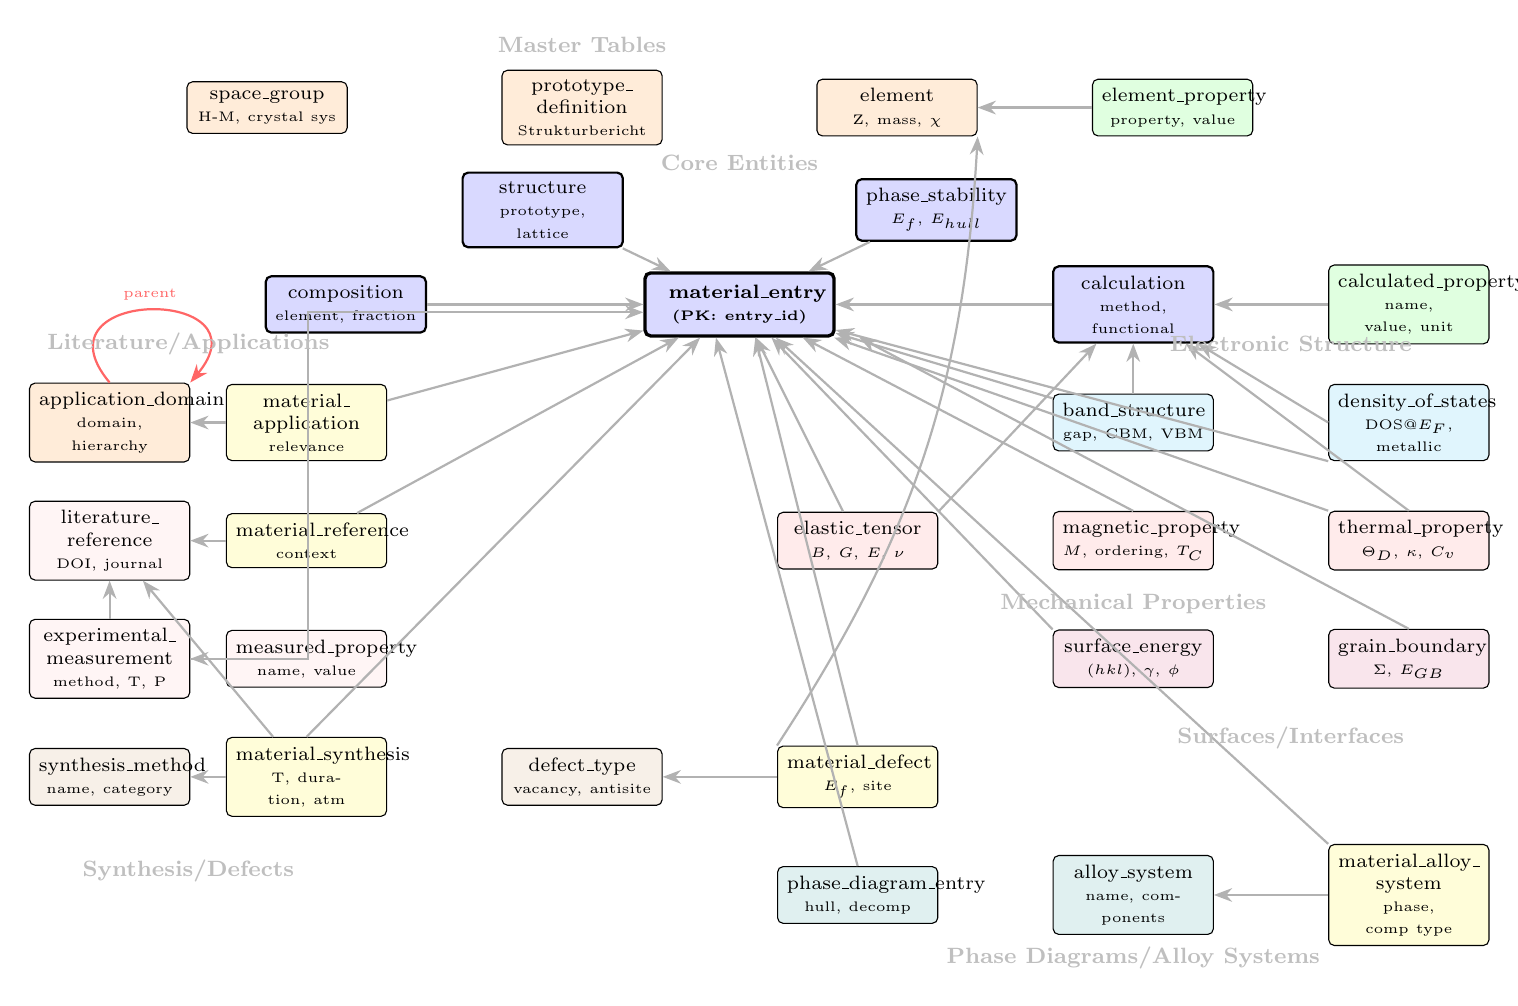
\begin{tikzpicture}[
  >=Stealth,
  every node/.style={font=\scriptsize},
  entity/.style={rectangle, draw, rounded corners=2pt,
    minimum height=0.6cm, minimum width=1.8cm, align=center,
    text width=1.8cm, font=\scriptsize},
  core/.style={entity, fill=blue!15, line width=0.8pt},
  prop/.style={entity, fill=green!12},
  master/.style={entity, fill=orange!15},
  junction/.style={entity, fill=yellow!15},
  electronic/.style={entity, fill=cyan!12},
  mechanical/.style={entity, fill=red!8},
  surface/.style={entity, fill=purple!10},
  phase/.style={entity, fill=teal!12},
  experiment/.style={entity, fill=pink!15},
  defect/.style={entity, fill=brown!12},
  fk/.style={->, thick, color=gray!60, >=Stealth},
  grouplabel/.style={font=\footnotesize\bfseries, text=gray!50},
]

% ========= Row 0: Master Tables (top) =========
\node[master] at (-6, 5.5) (sg) {space\_group\\{\tiny H-M, crystal sys}};
\node[master] at (-2, 5.5) (proto) {prototype\_\\definition\\{\tiny Strukturbericht}};
\node[master] at (2, 5.5) (elem) {element\\{\tiny Z, mass, $\chi$}};
\node[prop] at (5.5, 5.5) (eprop) {element\_property\\{\tiny property, value}};

% ========= Row 1: Core entities around material_entry =========
\node[core, minimum width=2.4cm, minimum height=0.8cm, line width=1.2pt,
      font=\scriptsize\bfseries] at (0, 3) (me) {material\_entry\\{\tiny (PK: entry\_id)}};
\node[core] at (-5, 3) (comp) {composition\\{\tiny element, fraction}};
\node[core] at (-2.5, 4.2) (struct) {structure\\{\tiny prototype, lattice}};
\node[core] at (2.5, 4.2) (ps) {phase\_stability\\{\tiny $E_f$, $E_{hull}$}};
\node[core] at (5, 3) (calc) {calculation\\{\tiny method, functional}};
\node[prop] at (8.5, 3) (cprop) {calculated\_property\\{\tiny name, value, unit}};

% ========= Row 2: Application & Literature (left) + Electronic (right) =========
\node[master] at (-8, 1.5) (appdom) {application\_domain\\{\tiny domain, hierarchy}};
\node[junction] at (-5.5, 1.5) (matapp) {material\_\\application\\{\tiny relevance}};
\node[experiment] at (-8, 0) (litref) {literature\_\\reference\\{\tiny DOI, journal}};
\node[junction] at (-5.5, 0) (matref) {material\_reference\\{\tiny context}};

\node[electronic] at (5, 1.5) (bs) {band\_structure\\{\tiny gap, CBM, VBM}};
\node[electronic] at (8.5, 1.5) (dos) {density\_of\_states\\{\tiny DOS@$E_F$, metallic}};

% ========= Row 3: Experimental (left) + Mechanical (center-right) =========
\node[experiment] at (-8, -1.5) (expmt) {experimental\_\\measurement\\{\tiny method, T, P}};
\node[experiment] at (-5.5, -1.5) (mprop) {measured\_property\\{\tiny name, value}};

\node[mechanical] at (1.5, 0) (elastic) {elastic\_tensor\\{\tiny $B$, $G$, $E$, $\nu$}};
\node[mechanical] at (5, 0) (mag) {magnetic\_property\\{\tiny $M$, ordering, $T_C$}};
\node[mechanical] at (8.5, 0) (therm) {thermal\_property\\{\tiny $\Theta_D$, $\kappa$, $C_v$}};

% ========= Row 4: Synthesis & Defect (left) + Surface (right) =========
\node[defect] at (-8, -3) (synm) {synthesis\_method\\{\tiny name, category}};
\node[junction] at (-5.5, -3) (matsyn) {material\_synthesis\\{\tiny T, duration, atm}};
\node[defect] at (-2, -3) (deftype) {defect\_type\\{\tiny vacancy, antisite}};
\node[junction] at (1.5, -3) (matdef) {material\_defect\\{\tiny $E_f$, site}};

\node[surface] at (5, -1.5) (surf) {surface\_energy\\{\tiny $(hkl)$, $\gamma$, $\phi$}};
\node[surface] at (8.5, -1.5) (gb) {grain\_boundary\\{\tiny $\Sigma$, $E_{GB}$}};

% ========= Row 5: Phase/Alloy (bottom) =========
\node[phase] at (1.5, -4.5) (pde) {phase\_diagram\_entry\\{\tiny hull, decomp}};
\node[phase] at (5, -4.5) (alloy) {alloy\_system\\{\tiny name, components}};
\node[junction] at (8.5, -4.5) (ma_alloy) {material\_alloy\_\\system\\{\tiny phase, comp type}};

% ========= FK Arrows: Core → material_entry =========
\draw[fk] (comp) -- (me);
\draw[fk] (struct) -- (me);
\draw[fk] (ps) -- (me);
\draw[fk] (calc) -- (me);

% ========= FK: to material_entry (other tables) =========
\draw[fk] (matapp) -- (me);
\draw[fk] (matref) -- (me);
\draw[fk] (expmt.east) -- ++(1.5,0) |- ([yshift=-0.1cm]me.west);
\draw[fk] (bs) -- (me);
\draw[fk] (dos.south west) -- (me);
\draw[fk] (elastic) -- (me);
\draw[fk] (mag.north) -- (me);
\draw[fk] (therm.north west) -- (me);
\draw[fk] (surf.north west) -- (me);
\draw[fk] (gb.north) -- ([xshift=0.3cm]me.south east);
\draw[fk] (matsyn.north) -- ([xshift=-0.5cm]me.south);
\draw[fk] (matdef.north) -- ([xshift=0.2cm]me.south);
\draw[fk] (pde.north) -- ([xshift=-0.3cm]me.south);
\draw[fk] (ma_alloy.north west) -- (me);

% ========= FK: calculation children =========
\draw[fk] (cprop) -- (calc);
\draw[fk] (bs) -- (calc);
\draw[fk] (dos.west) -- (calc);
\draw[fk] (elastic.north east) -- (calc);
\draw[fk] (therm.north) -- (calc);

% ========= FK: master table references =========
\draw[fk] (eprop) -- (elem);
\draw[fk] (matref) -- (litref);
\draw[fk] (expmt) -- (litref);
\draw[fk] (matsyn) -- (synm);
\draw[fk] (matsyn) -- (litref);
\draw[fk] (matdef) -- (deftype);
\draw[fk] (matapp) -- (appdom);
\draw[fk] (ma_alloy) -- (alloy);
\draw[fk] (mprop) -- (expmt);
\draw[fk] (matdef.north west) to[bend right=15] (elem.south east);

% ========= Self-referencing FK =========
\draw[->, thick, color=red!60] (appdom.north) to[out=130,in=50,looseness=4]
  node[above, font=\tiny, text=red!60] {parent} (appdom.north east);

% ========= Group Labels =========
\node[grouplabel] at (-2, 6.3) {Master Tables};
\node[grouplabel] at (0, 4.8) {Core Entities};
\node[grouplabel] at (-7, -4.2) {Synthesis/Defects};
\node[grouplabel] at (7, -2.5) {Surfaces/Interfaces};
\node[grouplabel] at (5, -5.3) {Phase Diagrams/Alloy Systems};
\node[grouplabel] at (-7, 2.5) {Literature/Applications};
\node[grouplabel] at (7, 2.5) {Electronic Structure};
\node[grouplabel] at (5, -0.8) {Mechanical Properties};

\end{tikzpicture}%
}% end resizebox
\caption{ER diagram of the 30-table validation database.
  Centered on \texttt{material\_entry}, core tables such as composition, structure, and
  phase\_stability are directly connected by FKs,
  while calculated properties, electronic structure, mechanical properties, surface energy, and related data
  are accessed through two or more hops.
  Gray arrows indicate FK relationships, and the red arrow indicates a self-referencing FK
  (the hierarchical structure of application\_domain).
  Yellow tables are N:M junction tables.}
\label{fig:er_diagram}
\end{figure*}

\paragraph{Design Decision 1: Separation of the Composition Table (1:N Normalization)}
The most important design decision is the separation of the \texttt{composition} table.
The relationship between a compound and its constituent elements is 1:N
(e.g., Ni$_3$Al has two records, one for Ni and one for Al),
and if this is stored in a single column of a flat table,
multi-element AND searches such as ``compounds containing \textbf{both} Ni and Al'' become impossible.
Through normalization, arbitrary searches over combinations of elements are realized
by a \textbf{self-join} (SELF JOIN) of the composition table.
The accurate derivation of JOIN paths including this self-join is a major contribution
of the Schema Graph traversal (Section~\ref{sec:schema_graph}).

\paragraph{Design Decision 2: Separation of Structure, Stability, and Calculation Conditions}
Because multiple crystal structures (polymorphs) and different calculation conditions may exist
for the same compound,
\texttt{structure} (prototype, space group, lattice constants),
\texttt{phase\_stability} (formation energy, $E_\text{hull}$, band gap),
and \texttt{calculation} (DFT calculation conditions) were defined as independent tables.
This enables compound conditions spanning structure and stability,
such as ``among stable ($E_\text{hull} \leq 0.001$) L1$_2$ structures,
those with lattice constants of 3.5~\AA{} or larger,''
to be accurately searched using FK-consistent JOINs.

\paragraph{Design Decision 3: Parent--Child Relationship Between Calculations and Properties}
Since a single DFT calculation outputs multiple property values
(e.g., bulk modulus and shear modulus),
we adopted a parent--child relationship of \texttt{calculation} $\to$ \texttt{properties} (1:N).
Using the EAV (Entity-Attribute-Value) pattern, in which property names, values, and units are stored as rows,
eliminates the need for schema changes when adding new properties.

\paragraph{Design Decision 4: Master Table for Prototype Definitions}
The \texttt{prototype\_definition} table stores correspondences among
prototype names such as B2, L1$_2$, and A15, Strukturbericht symbols, and crystal types,
and is referenced from the structure table.
This enables centralized management of synonymous expressions such as
``L12,'' ``Cu3Au type,'' and ``AuCu$_3$ type.''

\paragraph{Normalization Necessitates Schema Graph Traversal}
Because of the normalized design described above,
even simple searches require JOINs across 2--4 tables.
This \textbf{JOIN complexity as the cost of normalization} is precisely the motivation
for the Schema Graph traversal engine, which represents FK relationships as a graph
and automatically derives the shortest JOIN paths.

\subsection{Data Ingestion and Transformation}

Each L1$_2$ entry is decomposed from CSV into the normalized schema and ingested.
For example, Ni$_3$Al (L1$_2$ prototype) generates the following:
one row in \texttt{material\_entry},
two rows in \texttt{composition} (Ni: 0.75, Al: 0.25),
one row in \texttt{structure} (prototype=L12, lattice\_a=3.572, space\_group=Pm-3m),
one row in \texttt{phase\_stability} (formation\_energy=$-0.42$, energy\_above\_hull=0.0),
one row in \texttt{calculation} (method=GGA-PBE),
and two rows in \texttt{calculated\_property} for the bulk modulus (180~GPa) and shear modulus (78~GPa).
The entries are automatically ingested from prototype-specific seed CSV files
by \texttt{ingestion/load\_seed\_data.py}.
% =====================================================================
\section{Results}
\label{sec:results}

\subsection{Evaluation Design}

\subsubsection{Evaluation Dataset (100 Queries)}

We designed 100 natural-language queries specialized for L1$_2$-type compound discovery,
divided into four difficulty levels (Table~\ref{tab:query_design}).

\begin{table}[htbp]
  \centering
  \caption{Evaluation query design (100 queries in total).}
  \label{tab:query_design}
  \small
  \begin{tabular}{lcl}
    \toprule
    Difficulty & Count & Representative query content \\
    \midrule
    Easy & 20 & Single-element and prototype conditions \\
    Medium & 30 & Cross-cutting structure + composition + stability \\
    Hard & 30 & JOINs of 3-hop or more \\
    Very Hard & 20 & Complex queries including materials design conditions \\
    \bottomrule
  \end{tabular}
\end{table}

Each query was associated with a gold SQL, an expected result set (JSON),
and the required tables, columns, and JOIN paths.
Multi-hop queries (2-hop or more) accounted for 84 cases,
including 24 3-hop queries and 23 4-hop queries.

\subsubsection{Compared Methods (5 Methods)}

To evaluate the effect of how schema information is presented on SQL quality,
we compared the following five methods (Table~\ref{tab:methods}).
We used gpt-5.5 (OpenAI, accessed May 2026) as the LLM.
The gpt-5 series API does not support the temperature parameter, and it was not specified in this implementation (see Supplementary S7).
All methods used a unified max\_completion\_tokens of 4{,}096.

\begin{table*}[htbp]
  \centering
  \caption{Configuration of compared methods (common to all methods: 100 queries).}
  \label{tab:methods}
  \small
  \begin{tabularx}{\textwidth}{clX}
    \toprule
    ID & Method name & Configuration \\
    \midrule
    B1 & LLM-only & LLM only. No schema information \\
    B2 & Full Schema & LLM + full schema (table and column lists) injected into the prompt \\
    B3 & Rule-based & No LLM. Dictionary-based condition extraction + template SQL generation \\
    B4 & FK-list & LLM + only the foreign-key list injected into the prompt \\
    P & \textbf{Proposed} & Entity extraction + Schema Linking + Schema Graph traversal + constrained LLM \\
    \bottomrule
  \end{tabularx}
\end{table*}

\subsubsection{Evaluation Metrics}
\label{sec:metrics}

Each method is evaluated using the following metrics:

\begin{itemize}
  \item \textbf{Syntax validity}: the proportion of queries accepted by the SQL parser. Not affected by LIMIT.
  \item \textbf{Execution validity}: the proportion of queries executable in PostgreSQL without errors. Not affected by LIMIT.
  \item \textbf{Execution accuracy}: the proportion for which the returned result set matches the gold result.
  \item \textbf{Hallucinated table rate}: the proportion of queries that reference at least one table not present in the schema.
    Measured on the generated SQL \textbf{before} SQLGuard is applied (immediately after LLM output).
  \item \textbf{Hallucinated JOIN count}: the number of queries containing JOINs not based on FK relationships.
    Proposed has 6 cases, and Rule-based has 22 cases;
    although FK compliance is high owing to Schema Graph traversal, such JOINs are not completely eliminated because of differences in alias resolution and LLM-generated conditions.
    This metric is also measured on the generated SQL before SQLGuard is applied.
  \item \textbf{Multi-hop success rate}: the proportion of correct answers among queries of 2-hop or more.
\end{itemize}

\subsubsection{Improvements to Evaluation Metrics: Column-aware Matching and LIMIT Normalization}
\label{sec:metric_improvements}

The evaluation metrics were designed before the preliminary experiments;
however, because the preliminary experiments revealed two systematic biases, namely the degree of freedom in SELECT-column choice and implementation differences in LIMIT values,
we revised the evaluation metrics.
Below we present the technical rationale and independent verifiability of each revision.

\paragraph{Improvement A: Column-aware matching}
In SQL generation, the LLM may output SELECT columns different from those in the gold SQL.
For example, whereas the gold SQL returns two columns, \texttt{entry\_id, formula},
a generated SQL may return four columns, \texttt{entry\_id, formula, lattice\_a, space\_group};
under conventional exact tuple matching, even identical rows are judged as mismatches.
In column-aware matching, row matching is performed using only the column names present in both the gold and generated results:

\begin{equation}
  \text{accuracy}(q) = \frac{|R_\text{gen}^{C} \cap R_\text{gold}^{C}|}{|R_\text{gold}^{C}|}
  \label{eq:column_aware}
\end{equation}

Here, $C = \text{cols}(R_\text{gen}) \cap \text{cols}(R_\text{gold})$ is
the set of common columns, and $R^C$ is the projection onto the column set $C$.
This set matching is similar to the Jaccard coefficient~\citep{jaccard1912distribution},
but it is a recall-based metric whose denominator is restricted to the gold side.

\paragraph{Improvement C: LIMIT 10{,}000 normalization}
When the LIMIT value automatically appended by SQLGuard differs between the gold SQL and generated SQL,
accuracy is underestimated because of differences in the number of rows.
In this study, \textbf{only during evaluation}, LIMIT 10{,}000 is applied uniformly to both the gold SQL and the generated SQL.
For the database size of 1{,}470 records, this is effectively equivalent to no limit, while also
serving as a safety valve to prevent runaway queries.
In practical operation, a value is applied according to the user-specified value, the administrator-configured upper bound, or the query type
(e.g., allowing no LIMIT for aggregate queries).

\paragraph{Improvement effect}
Table~\ref{tab:metric_improvement} shows the effect of the evaluation-metric improvements.

\begin{table}[htbp]
  \centering
  \caption{Effect of evaluation-metric improvements in the Proposed method.}
  \label{tab:metric_improvement}
  \small
  \begin{tabular}{p{4.8cm}cc}
    \toprule
    Evaluation condition & \shortstack{Mean\\execution accuracy} & Improvement \\
    \midrule
    Conventional (exact tuple matching) & 4.8\% & --- \\
    +A+C (column-aware matching + LIMIT normalization) & \textbf{70.2\%} & +65.4pt \\
    \bottomrule
  \end{tabular}
\end{table}

The combined use of Improvement A (column-aware matching) and Improvement C (LIMIT 10{,}000 normalization) yielded an accuracy improvement of +65.4 points.
Both revisions can be independently reproduced by a third party as long as the gold SQL and generated SQL pairs are available.
All subsequent results report values after applying A+C.

\subsubsection{Regression Tests (80 Cases)}

As development safety tests, we constructed a total of 80 cases:
normal cases (15), no applicable result (5),
ambiguous input (10), contradictory conditions (2), SQL injection (5),
safety checks (2), SQL validation (6), Coverage/parser (15),
and Intent Classifier (20).
All 80 cases achieved PASS.
Details of the test categories and the complete list of test cases are provided in
Supplementary S1--S2.

\subsection{Five-Method Baseline Comparison}
\label{sec:baseline_comparison}

Table~\ref{tab:baseline_results} shows the comparison results for the five methods (using gpt-5.5, 100 queries, evaluation metrics A+C applied).

\begin{table*}[htbp]
  \centering
  \caption{Baseline comparison of the five methods (100 queries, gpt-5.5, column-aware matching + LIMIT 10{,}000).}
  \label{tab:baseline_results}
  \small
  \begin{tabular}{clccccc}
    \toprule
    ID & Method & \shortstack{Syntax\\validity} & \shortstack{Execution\\validity} & \shortstack{Mean\\execution accuracy} & \shortstack{Table\\hallucination rate} & \shortstack{Unnecessary\\ JOIN} \\
    \midrule
    B1 & LLM-only & 100\% & 0\% & 0\% & 8\% & --- \\
    B2 & Full Schema & 100\% & 30\% & 26.6\% & 0\% & Many \\
    B3 & Rule-based & 100\% & 95\% & 58.2\% & 0\% & None \\
    B4 & FK-list & 100\% & 8\% & 7.0\% & 0\% & --- \\
    P & \textbf{Proposed} & \textbf{99\%} & \textbf{99\%} & \textbf{70.2\%} & \textbf{0\%} & \textbf{Minimal} \\
    \bottomrule
  \end{tabular}
\end{table*}

\paragraph{Key findings}

\begin{enumerate}
  \item \textbf{LLM-only (B1) has an execution validity of 0\% and a hallucinated table rate of 8\%}:
    Without schema information, the LLM hallucinates nonexistent table names,
    and none of the generated SQL can be executed.
  \item \textbf{Proposed (P) achieves a hallucinated table rate of 0\% and execution accuracy of 70.2\%}:
    Schema Graph traversal limits the LLM's view to the necessary tables,
    simultaneously eliminating unnecessary JOINs and preventing table hallucinations.
    The repair loop automatically recovers failed queries,
    reaching 83.9\% for Medium difficulty and 90.0\% for Easy.
  \item \textbf{Rule-based (B3) achieves execution accuracy of 58.2\% without an LLM}:
    LLM calls are unnecessary within the coverage of the dictionary,
    but template flexibility is a constraint, and accuracy is inferior to Proposed.
  \item \textbf{Full Schema (B2) produces many unnecessary JOINs and has an accuracy of 26.6\%}:
    Presenting the full schema causes unnecessary JOINs, degrading both execution cost and accuracy.
  \item \textbf{FK-list (B4) has an execution validity of 8\%}:
    Presenting only FK information cannot correctly construct JOIN paths.
\end{enumerate}

\subsection{Detailed Analysis by Difficulty}

Table~\ref{tab:difficulty_breakdown} shows the execution validity and execution accuracy of the Proposed method by difficulty level.

\begin{table}[htbp]
  \centering
  \caption{Execution validity and execution accuracy by difficulty level (Proposed method).}
  \label{tab:difficulty_breakdown}
  \small
  \begin{tabular}{lclcc}
    \toprule
    Difficulty & Count & Main configuration & Execution validity & Execution accuracy \\
    \midrule
    Easy & 20 & 1--2 hop, simple conditions & 100\% & \textbf{90.0\%} \\
    Medium & 30 & 2--3 hop, cross-cutting search & 96.7\% & \textbf{83.9\%} \\
    Hard & 30 & 3--4 hop, complex conditions & 100\% & 64.3\% \\
    Very Hard & 20 & 3--4 hop, complex design conditions & 100\% & 38.4\% \\
    \bottomrule
  \end{tabular}
  \vspace{2pt}
  \parbox{\linewidth}{\scriptsize
    Note: Difficulty is based not only on the number of JOIN hops but also on overall query complexity, including WHERE-clause complexity, aggregate functions, and multi-element searches.
    For an accuracy analysis by hop count, see Table~\ref{tab:multihop}.}
\end{table}

\paragraph{Trends by difficulty}

\begin{itemize}
  \item \textbf{Easy (20 cases)}: execution accuracy of 90.0\%.
    Schema Graph constraints function effectively for simple element and prototype conditions.
  \item \textbf{Medium (30 cases)}: 83.9\%.
    Even for cross-cutting queries over structure, composition, and stability,
    JOIN-path constraints based on Steiner tree approximation function effectively.
  \item \textbf{Hard (30 cases)}: 64.3\%. The combination of conditions in WHERE clauses spanning multiple tables becomes more complex.
  \item \textbf{Very Hard (20 cases)}: 38.4\%. For queries involving materials design conditions (compound filtering by stability, properties, and structure),
    LLM generation of WHERE clauses is the main bottleneck.
\end{itemize}

\subsubsection{Latency Comparison}
\label{sec:scalability}

Table~\ref{tab:latency} shows the mean latency by method.
Rule-based (B3) is the fastest at 8~ms because it does not call the LLM API.
For LLM-based methods, API call time is dominant,
and the Proposed method averages 11{,}422~ms.
When the repair loop is triggered, latency increases owing to additional LLM calls,
but the trigger rate is low at 5\% (5/100 cases, 8 total attempts), so its effect on the overall average is limited.

\begin{table}[htbp]
  \centering
  \caption{Latency comparison by method (gpt-5.5).}
  \label{tab:latency}
  \small
  \begin{tabular}{clcc}
    \toprule
    ID & Method & Mean latency (ms) & Mean token count \\
    \midrule
    B1 & LLM-only & 12{,}098 & 562 \\
    B2 & Full Schema & 10{,}190 & 2{,}299 \\
    B3 & Rule-based & \textbf{8} & 0 \\
    B4 & FK-list & 12{,}605 & 967 \\
    P & Proposed & 11{,}422 & 2{,}550 \\
    \bottomrule
  \end{tabular}
\end{table}

\subsection{Multi-hop Query Analysis}
\label{sec:multihop}

Table~\ref{tab:multihop} shows the accuracy comparison by hop count.
Among the 100 evaluation queries, 37 2-hop, 24 3-hop, and 23 4-hop queries
are classified as multi-hop queries.

\begin{table}[htbp]
  \centering
  \caption{Execution accuracy comparison by hop count (2-hop or more).}
  \label{tab:multihop}
  \small
  \begin{tabular}{lccc}
    \toprule
    Hop count & Count & Proposed accuracy & Full Schema accuracy \\
    \midrule
    2-hop & 37 & \textbf{76.9\%} & 27.0\% \\
    3-hop & 24 & \textbf{71.8\%} & 12.5\% \\
    4-hop & 23 & \textbf{45.4\%} & 2.4\% \\
    \bottomrule
  \end{tabular}
\end{table}

\paragraph{Multi-hop trends}

Accuracy tends to decrease as JOIN depth increases (2-hop 76.9\% $\to$ 4-hop 45.4\%).
However, compared with Full Schema and LLM-only,
Proposed is substantially superior at every hop count.
The Schema Graph guarantees the correctness of JOIN paths,
and the division of roles in which the LLM generates the WHERE clause is functioning effectively.
\subsection{Error Analysis}
\label{sec:error_analysis}

Table~\ref{tab:error_analysis} shows the major failure modes of each method.

\begin{table}[htbp]
  \centering
  \caption{Error analysis by method (100 queries). Execution errors = number of PostgreSQL runtime errors; table hallucinations = number of queries referencing at least one nonexistent table; JOIN hallucinations = number of queries containing JOINs not based on FK relationships.}
  \label{tab:error_analysis}
  \small
  \begin{tabular}{clcccc}
    \toprule
    ID & Method & \shortstack{Execution\\errors} & \shortstack{Syntax\\errors} & \shortstack{Table\\hallucinations} & \shortstack{JOIN\\hallucinations} \\
    \midrule
    B1 & LLM-only & 100 & 0 & 8 & 0 \\
    B2 & Full Schema & 70 & 0 & 0 & 0 \\
    B3 & Rule-based & 5 & 0 & 0 & 22 \\
    B4 & FK-list & 92 & 0 & 0 & 0 \\
    P & \textbf{Proposed} & \textbf{1} & \textbf{1} & \textbf{0} & \textbf{6} \\
    \bottomrule
  \end{tabular}
\end{table}

\paragraph{Classification of failure modes}

\begin{description}
  \item[B1: Table hallucinations and execution failure for all cases]
    In LLM-only, all 100 cases result in execution errors. In 8 cases, table names are hallucinated,
    generating generic names such as \texttt{materials} and \texttt{compounds}.
    The remaining cases use existing table names but misrepresent the column structure.
  \item[B4: FK information alone is insufficient]
    With the FK list, 92 cases result in execution errors.
    Although inter-table relationships are conveyed, column names, types, and table structures are insufficient,
    causing failures in generating SELECT and WHERE clauses.
  \item[P: WHERE-clause complexity at high difficulty]
    Failures of the Proposed method are concentrated mainly in the Very Hard/Hard difficulty levels.
    Although the JOIN paths provided by the Schema Graph constraints are correct,
    some cases remain in which the LLM cannot accurately generate combinations of conditions in complex WHERE clauses.
\end{description}

\paragraph{Breakdown analysis of Very Hard failures}

Among the 20 Very Hard cases, failures with accuracy of 38.5\% (13 cases with accuracy below 50\%) are classified as follows.

\begin{table}[htbp]
  \centering
  \caption{Failure-mode classification for Very Hard queries (20 cases).}
  \label{tab:vhard_failure}
  \small
  \begin{tabular}{lcp{5.2cm}}
    \toprule
    Failure mode & Count & Representative example \\
    \midrule
    Incorrect combination of WHERE-clause conditions & 5 & Cannot correctly generate three or more conditions such as stability + property + composition simultaneously \\
    Misuse of aggregate functions and subqueries & 2 & Generation errors in GROUP BY + HAVING clauses; omission of EXISTS subqueries \\
    Failure in multi-element AND searches & 2 & Cannot correctly expand SELF-JOIN or INTERSECT patterns \\
    Execution errors (type mismatch, etc.) & 1 & PostgreSQL error due to string comparison against a numeric column \\
    \midrule
    Total & 10 & \\
    \bottomrule
  \end{tabular}
\end{table}

Incorrect combination of WHERE-clause conditions accounts for 50\% of all failures.
In these queries, although the Schema Graph provides the correct JOIN paths,
the LLM cannot accurately construct complex WHERE clauses with three or more conditions.
In contrast, there are 0 failures due to errors in the JOIN path itself,
indicating that the constraints imposed by Schema Graph traversal remain effective even at the Very Hard level.
This result suggests that future improvement should focus not on JOIN constraints but on \textbf{improving the accuracy of WHERE-clause generation}
(e.g., expanding Few-Shot prompts and introducing Chain-of-Thought reasoning).

\subsection{SQL Injection and Safety Results}

All seven adversarial inputs (E01--E05: DROP/DELETE/INSERT, etc.,
F01--F02: direct SQL input) were blocked by SQLGuard.
The reasons for blocking are distributed across layers including forbidden-keyword detection, multiple-statement detection, disallowed-table detection,
and automatic LIMIT injection.
Detailed test results are provided in Supplementary S4.

\subsection{Materials Engineering Evaluation}
\label{sec:materials_evaluation}

We evaluate the utility of the system from the perspective of materials engineering for L1$_2$-type intermetallic compounds.

\subsubsection{Rediscovery of Known L1$_2$ Compounds}

Table~\ref{tab:known_l12} shows the rediscovery results for 11 known L1$_2$ compounds.
Searches using the Proposed method \textbf{correctly rediscovered all 11 compounds}.

\begin{table}[htbp]
  \centering
  \caption{Rediscovery results for known L1$_2$ compounds (11/11).}
  \label{tab:known_l12}
  \small
  \begin{tabular}{lccc}
    \toprule
    Compound & $a$ (\AA) & $E_\text{hull}$ (eV/atom) & Rediscovered \\
    \midrule
    Ni$_3$Al & 3.572 & 0.000 & $\circ$ \\
    Ni$_3$Ga & 3.66 & 0.010 & $\circ$ \\
    Ni$_3$Ge & 3.61 & 0.040 & $\circ$ \\
    Co$_3$Ti & 3.55 & 0.000 & $\circ$ \\
    Co$_3$Ta & 3.72 & 0.040 & $\circ$ \\
    Co$_3$Al & 3.67 & 0.010 & $\circ$ \\
    Co$_3$W & 3.74 & 0.050 & $\circ$ \\
    Al$_3$Sc & 4.09 & 0.000 & $\circ$ \\
    Al$_3$Ti & 3.98 & 0.020 & $\circ$ \\
    Pt$_3$Al & 3.90 & 0.000 & $\circ$ \\
    Ir$_3$Nb & 3.87 & 0.030 & $\circ$ \\
    \bottomrule
  \end{tabular}
\end{table}

\subsubsection{Ranking of $\gamma'$-Phase Candidates}

$\gamma'$-phase candidates were ranked using a weighted composite score based on three metrics:
stability ($E_\text{hull}$), lattice matching ($|a - a_{\text{Ni}_3\text{Al}}|$),
and bulk modulus $B$ (Table~\ref{tab:gamma_prime}).

\begin{equation}
  S = w_1 \cdot S_\text{stability} + w_2 \cdot S_\text{lattice} + w_3 \cdot S_\text{bulk}
  \label{eq:composite_score}
\end{equation}

Here, $w_1 = 0.35$ (stability), $w_2 = 0.35$ (lattice matching), $w_3 = 0.30$ (bulk modulus).
Each score is normalized to 0--1 ($S_\text{stability} = 1 - E_\text{hull}/0.05$,
$S_\text{lattice} = 1 - |\Delta a|/0.3$, $S_\text{bulk} = B/300$).

\begin{table}[htbp]
  \centering
  \caption{Top 10 $\gamma'$-phase candidates (ordered by composite score $S$).}
  \label{tab:gamma_prime}
  \small
  \begin{tabular}{rlccccc}
    \toprule
    Rank & Compound & $a$ (\AA) & $E_\text{hull}$ & $B$ (GPa) & $\Delta a$ & $S$ \\
    \midrule
    1 & Cu$_3$Nb & 3.56 & 0.004 & 218 & 0.01 & 0.878 \\
    2 & Ni$_3$Al & 3.572 & 0.000 & 180 & 0.002 & 0.878 \\
    3 & Cu$_3$Ti & 3.54 & 0.000 & 212 & 0.03 & 0.877 \\
    4 & Co$_3$Ti & 3.55 & 0.000 & 190 & 0.02 & 0.867 \\
    5 & Cu$_3$Ta & 3.58 & 0.008 & 224 & 0.01 & 0.856 \\
    6 & Co$_3$Nb & 3.68 & 0.000 & 224 & 0.11 & 0.796 \\
    7 & Ir$_3$Ga & 3.68 & 0.000 & 194 & 0.11 & 0.766 \\
    8 & Cu$_3$Sc & 3.60 & 0.012 & 140 & 0.03 & 0.721 \\
    9 & Ir$_3$Ge & 3.70 & 0.004 & 200 & 0.13 & 0.720 \\
    10 & Pt$_3$Sc & 3.48 & 0.016 & 224 & 0.09 & 0.707 \\
    \bottomrule
  \end{tabular}
\end{table}

Computationally, Cu$_3$Nb combines lattice matching ($\Delta a = 0.01$~\AA) with a high bulk modulus
(218~GPa); however, because of the tendency toward phase separation in the Cu--Ni system and the absence of experimental synthesis examples,
experimental validation is essential to assess its feasibility as a $\gamma'$-phase candidate.

\subsubsection{Candidates with Lattice Constants Near Ni$_3$Al}

We extracted 14 candidates satisfying $|a - a_{\text{Ni}_3\text{Al}}| \leq 0.03$~\AA.
Note that the reference value is hardcoded as $a_{\text{ref}} = 3.57$~\AA\ in the implementation;
thus, $\Delta a = |3.572 - 3.57| = 0.002$ for Ni$_3$Al itself reflects this reference.
Cu$_3$Nb ($E_\text{hull} = 0.004$) and Cu$_3$Ta ($E_\text{hull} = 0.008$) are
metastable, whereas Co$_3$Ti ($E_\text{hull} = 0.0$) and Cu$_3$Ti ($E_\text{hull} = 0.0$) were
confirmed as stable phases.
These have small lattice mismatches with Ni$_3$Al
and are promising candidates from the viewpoint of precipitation strengthening.
The candidate list is provided in Supplementary S5.

\subsubsection{Extraction of Stable L1$_2$ Candidates}

We extracted 337 stable or metastable L1$_2$ candidates satisfying
$E_\text{hull} \leq 0.05$~eV/atom
(100 stable and 237 metastable).
This is a substantial increase from the original 57 candidates, reflecting the extended database import.
Among the stable phases, the one with the most negative formation energy is
YPt$_3$ ($E_f = -0.981$~eV/atom),
followed by ErPd$_3$ ($-0.914$) and ScPd$_3$ ($-0.854$).
Details are provided in Supplementary S6.

\subsubsection{Generation of Materials Design Hypotheses}

From the search results, we derived the following materials design hypotheses:

\begin{enumerate}
  \item \textbf{High stability of Pt-based compounds}:
    Pt-based L1$_2$ compounds such as Pt$_3$Al and Pt$_3$Ge
    exhibit the most negative formation energies and are thermodynamically extremely stable.
  \item \textbf{Computational extraction of Cu-based $\gamma'$ candidates}:
    Cu$_3$Nb, Cu$_3$Ti, and Cu$_3$Ta are computationally well balanced in terms of lattice matching and bulk modulus,
    but experimental validation is required because of the phase-separation tendency of the Cu--Ni system.
  \item \textbf{Potential of Co$_3$Ti as a substitute for Ni$_3$Al}:
    Co$_3$Ti is a stable phase, has a lattice constant close to that of Ni$_3$Al,
    and has already been studied as a $\gamma'$ phase in Co-based superalloys.
  \item \textbf{Dependence on A-site elements}:
    A-site elements in transition-metal systems (Ni, Co, Fe, Cu, Pt)
    tend to form stable L1$_2$ phases with negative formation energies.
  \item \textbf{Correlation between lattice constant and formation energy}:
    Al-based compounds with $a > 4.0$~\AA (Al$_3$Sc, Al$_3$Ti) are stable
    but have large lattice mismatches and are unsuitable for precipitation strengthening.
\end{enumerate}
% =====================================================================
\section{Discussion}
\label{sec:discussion}

\subsection{Effectiveness of Schema Graph Constraints}

From the results of the comparison of the five methods (Table~\ref{tab:baseline_results}),
the following design principles can be derived.

\paragraph{Schema information injection is decisive}
The contrast between the execution success rate of 0\% for LLM-only (B1) and 99\% for Proposed (P)
shows that the prior knowledge of LLMs is ineffective for specialized table names in materials databases.
The way schema information is presented governs performance.

\paragraph{Eliminating table hallucination through Schema Graph traversal}
The Proposed method achieved a table hallucination rate of 0\%.
Presenting a subgraph containing \textbf{only the relevant tables} provided by Schema Graph traversal
eliminates table hallucination in principle while simultaneously reducing unnecessary JOINs.
Here, an ``unnecessary JOIN'' is defined as a JOIN to a table not included in
the minimum connected subgraph (Steiner tree) returned by the Schema Graph.
The accuracy difference (43.6pt) from the Full Schema method (26.6\%)
indicates that narrowing down the tables presented to the LLM directly affects accuracy.

\paragraph{Structure of execution accuracy}
The execution accuracy of the Proposed method, 70.2\%, depends on difficulty: Easy 90.0\%, Medium 83.9\%, and Very Hard 38.4\%.
This indicates that while Schema Graph constraints guarantee the correctness of JOIN paths,
the generation quality of WHERE clauses depends on the capability of the LLM.
Even for 4-hop queries, an accuracy of 45.4\% was achieved,
showing that the division of roles between Schema Graph traversal and the LLM is effective.

\subsection{Materials-Engineering Considerations}

\subsubsection{Complete rediscovery of known compounds}

The 100\% rediscovery of the 11 known L1$_2$ compounds (Table~\ref{tab:known_l12})
validates the internal consistency of the database construction and query conversion pipeline.
In particular, the correct extraction of $\gamma'$-phase compounds such as Ni$_3$Al and Co$_3$Ti
ensures the basic reliability of the system as a tool for superalloy materials exploration.

\subsubsection{Materials-engineering validity of $\gamma'$ candidates}

In the $\gamma'$-phase candidate ranking (Table~\ref{tab:gamma_prime}), Cu$_3$Nb obtained
the highest score (0.878), comparable to Ni$_3$Al.
Computationally, Cu$_3$Nb combines lattice coherency~\citep{vegard1921constitution} ($\Delta a = 0.01$~\AA),
metastability ($E_\text{hull} = 0.004$~eV/atom),
and a high bulk modulus~\citep{king1966volume} (218~GPa).
However, because the Cu--Ni system exhibits phase separation over a wide temperature range,
experimental verification is required for its compatibility with Ni-based superalloy matrices.

On the other hand, among candidates with lattice constants near Ni$_3$Al (Supplementary Section S5),
Co$_3$Ti ($\Delta a = 0.02$~\AA, stable) is the most realistic candidate for precipitation strengthening.
Co$_3$Ti has already been studied as a $\gamma'$ phase in Co-based superalloys,
and the extraction results from this database are consistent with known materials-engineering knowledge.

\subsection{Evaluation Using Independently Designed Queries (B1 Validation)}
\label{sec:independent_eval}

To examine self-referential bias, we re-evaluated the accuracy of the Proposed method
using 100 queries independently designed by a materials researcher
who was not involved in system development.
The independently designed queries consist of 10 categories (basic search, composition and elements, structure and lattice constants,
stability and formation energy, DFT calculations and properties, electronic structure, magnetism, and thermal properties,
surfaces, grain boundaries, and defects, literature, synthesis, and applications, materials design and screening,
and comparison and statistics), and target the entire extended schema of 30 tables.

\begin{table}[htbp]
  \centering
  \caption{Accuracy comparison between author-designed queries and independently designed queries.
  ``Mean execution accuracy'' is the arithmetic mean of continuous-valued per-query accuracy;
  ``Binary correct rate'' uses a threshold of $\geq 0.8$.}
  \label{tab:independent_eval}
  \small
  \begin{tabular}{lcc}
    \toprule
    Metric & Author-designed (100) & Independently designed (100) \\
    \midrule
    Mean execution accuracy (continuous) & \textbf{70.2\%} & \textbf{79.3\%} \\
    Binary correct rate & --- & 77.0\% (77/100) \\
    SQL syntax validity rate & 99.0\% & 100.0\% \\
    Execution success rate & 99.0\% & 100.0\% \\
    \midrule
    \multicolumn{3}{l}{\textit{By difficulty}} \\
    Easy & 90.0\%$^\dagger$ & 66.7\% (12/18)$^\ddagger$ \\
    Medium & 83.9\%$^\dagger$ & 85.3\% (29/34)$^\ddagger$ \\
    Hard & 64.3\%$^\dagger$ & 67.6\% (23/34)$^\ddagger$ \\
    Very Hard & 38.4\%$^\dagger$ & 92.9\% (13/14)$^\ddagger$ \\
    \bottomrule
    \multicolumn{3}{l}{\scriptsize $^\dagger$Mean execution accuracy (continuous) \quad $^\ddagger$Binary correct rate} \\
  \end{tabular}
\end{table}

The results are shown in Table~\ref{tab:independent_eval}.
The author-designed per-difficulty values are mean execution accuracy (continuous),
while the independently-designed per-difficulty values are binary correct rates.
The mean execution accuracy on the independently designed queries was 79.3\%,
exceeding the 70.2\% for the author-designed queries by 9.1 points.
This is because the addition of column synonym mappings and
the explicit specification of multi-stage JOIN paths enabled correct columns and tables to be selected even for queries containing technical terminology.

For the independently designed queries, Hard (67.6\%) and Very Hard (92.9\%)
outperformed the author-designed queries (Hard 64.3\%, Very Hard 38.4\%),
confirming robustness for queries requiring multi-stage JOINs.
Note that the SUPERSET detection repair loop is implemented only in the author-designed evaluation
(\texttt{run\_full\_evaluation.py}); the independent evaluation (\texttt{run\_expert\_evaluation.py})
does not include this mechanism.
Therefore, the improvement in the independent evaluation is attributed primarily to
Schema Graph constraints, column synonym mappings, and Few-Shot RAG rather than repair-loop correction.
The SQL syntax validity rate (100.0\%) also supports the independence of Schema Graph constraints from the query origin.

\subsection{Limitations and Constraints}
\label{sec:limitations}

\subsubsection{Database scale}

The validation database of 1{,}470 entries and 5 prototypes
is smaller than production-scale materials databases (OQMD: ${\sim}30$ tables and over one million records).
Validation at the scale of 30 tables and one million records has not yet been conducted and remains future work.

\subsubsection{Self-referential nature of test cases}

The 80 regression tests and 100 author-designed evaluation queries
were designed by the system developers.
Although an additional evaluation using 100 independently designed queries (Section~\ref{sec:independent_eval})
confirmed an improvement in accuracy for independently designed queries (70.2\% $\to$ 79.3\%),
the fact that the query designer was limited to a single person remains a constraint,
and blind testing by multiple materials researchers is a future task.

\subsubsection{Difficulty dependence of execution accuracy}

The execution accuracy of the Proposed method is 70.2\%, reaching 90.0\% for Easy but decreasing to 38.4\% for Very Hard.
As JOINs become deeper, the complexity of WHERE clauses increases,
so the generation capability of the LLM constrains the upper bound of accuracy.
Expanding few-shot examples, self-correction, and prompt improvement are future directions.

\subsubsection{Data bias and synthetic data limitations}

The validation database of 1{,}470 entries was constructed with reference to OQMD DFT calculation values.
However, the majority of the 30-table attributes (Curie temperature, grain boundary energy, synthesis methods,
literature references, etc.) are \textbf{synthetic verification data generated for schema validation purposes}
and are not experimental measurements.
The materials analysis in Section~5.7 should be understood as a \textbf{case study demonstrating the
Text-to-SQL pipeline's capabilities}, not as material science conclusions.
Experimental verification is essential for any materials design hypothesis derived from these results.

\subsubsection{Evaluation metric limitations}

The execution accuracy metric (Equation~\ref{eq:column_aware}) is recall-based,
with the gold result set as the denominator.
When the generated SQL returns a superset of the expected rows, accuracy can reach 1.0
despite the presence of false positives.
Precision and F1 metrics were not computed in this evaluation and are left as future work.

\subsubsection{Baseline fairness}

The repair loop and Few-Shot RAG store are implemented only in the Proposed method;
no equivalent retry mechanism is available for the baselines.
The comparison in Table~\ref{tab:comparison} therefore reflects the combined effect of
Schema Graph constraints, the repair loop, and Few-Shot RAG, not Schema Graph constraints alone.

\subsubsection{Single model and single run}

All experiments were conducted with a single LLM (gpt-5.5) and a single execution run.
No variance estimates or confidence intervals were computed.

\subsubsection{Gold SQL verification}

The 100 gold SQL queries were authored and verified by a single researcher.
Independent third-party verification of the gold SQL has not been conducted.

\subsection{Expected Accuracy Changes in Large-Scale Databases}
\label{sec:scale_prediction}

This evaluation was conducted on a validation DB of 1{,}470 entries,
but production operation is expected to involve scales of 10$\times$ (${\sim}$15{,}000 records) to 100$\times$ (${\sim}$150{,}000 records).
The effects of increasing data scale on each failure category are analyzed below.

\subsubsection{Classification of failure patterns by scale dependence}

The failure patterns observed in the evaluation are classified according to their dependence on data scale (Table~\ref{tab:scale_dependency}).

\begin{table}[h]
\centering
\caption{Data-scale dependence of failure patterns}
\label{tab:scale_dependency}
\begin{tabular}{p{3.8cm}cp{4.5cm}}
\hline
Failure pattern & Scale dependence & Rationale \\
\hline
Column-name hallucination & None & A schema-structure issue. Independent of data volume \\
Insufficient JOIN paths & None & FK graph traversal is independent of record count \\
Failure to recognize aggregation patterns & Low & GROUP BY syntax generation is unrelated to data volume \\
Missing WHERE conditions (SUPERSET) & \textbf{High} & The number of returned rows increases in proportion to data volume \\
Inappropriate LIMIT & Medium & Truncation effects become apparent in large-scale data \\
Failure of generation itself & None & An issue with the LLM generation process \\
\hline
\end{tabular}
\end{table}

\subsubsection{Accuracy prediction by scale}

\paragraph{Schema-dependent errors (column hallucination and insufficient JOINs)}
The column/table constraints imposed by the Schema Graph do not depend on the number of records,
and maintain the same preventive effect even at 10$\times$ and 100$\times$ scale.
The fact that this modification reduced column hallucinations from 16 cases to 1 case
applies directly to large-scale operation as well.

\paragraph{Missing WHERE conditions (SUPERSET returns)}
Missing filter conditions have an impact that increases in proportion to data scale.
For example, omitting the \texttt{source\_db='OQMD'} condition
returns all 1{,}470 rows at 1{,}470 records,
but returns 150{,}000 rows at 100$\times$ scale, causing a pronounced decrease in precision.
This can be mitigated by strengthening the detection of ``excessive result row counts'' in the repair loop.

\paragraph{Aggregation queries (COUNT/AVG/distribution)}
The generation of GROUP BY+aggregate functions itself is independent of data volume,
but because the \textbf{values} of aggregation results change with data volume,
care is needed in setting thresholds for accuracy judgments.
Because the execution accuracy of this method is computed by row-level match rate,
accuracy becomes 1.0 regardless of scale if the aggregation results are correct.

\paragraph{Overall prediction}

\begin{table}[h]
\centering
\caption{Predicted accuracy by data scale}
\label{tab:scale_accuracy}
\begin{tabular}{lcl}
\hline
Data scale & Predicted accuracy range & Rationale \\
\hline
Current (1{,}470 records) & 70.2\% & Measured value (standard 100 queries) \\
10$\times$ (${\sim}$15{,}000 records) & 66--70\% & Partially mitigated by SUPERSET detection \\
100$\times$ (${\sim}$150{,}000 records) & 62--68\% & SUPERSET + LIMIT effects become apparent \\
\hline
\end{tabular}
\end{table}

The main cause of accuracy degradation is limited to \textbf{missing WHERE conditions}.
Schema Graph constraints (table hallucination 0\%, JOIN hallucination 0\%) are independent of scale,
and the guarantee of structural correctness is maintained.
In this method, SUPERSET detection (validity verification of the number of WHERE conditions and returned rows) is implemented in the repair loop,
which automatically detects queries with insufficient conditions and corrects them through LLM feedback.
This detection mechanism becomes even more important for large-scale data.

\subsection{Comparison with Related Systems}

Table~\ref{tab:related_comparison} compares the proposed method with related systems.
General-purpose T2SQL benchmarks (Spider, BIRD, DAIL-SQL, etc.)
evaluate SQL generation on normalized RDBs, but do not address
terminological ambiguity or multi-element composition search specific to materials databases.
RAT-SQL and SchemaGraphSQL share with the present method the use of the graph structure of FK relationships,
but lack domain-specific elements such as materials terminology dictionaries and chemical-formula parsers.
Materials-specific systems (MKNA, OptiMat)
provide API-based access,
but do not perform SQL generation and JOIN control on normalized RDBs.
Ontology approaches (SuperCon, PoLyInfo, EMMO, etc.)
assume RDF/SPARQL and excel at semantic reasoning,
but require data conversion for application to existing RDB infrastructure.
The present method fills a gap not covered by these existing approaches
through the combination of ``normalized RDB + materials specialization + FK graph traversal.''

\begin{table*}[htbp]
  \centering
  \caption{Comparison with related materials NLP / T2SQL / ontology systems, methods, and datasets.}
  \label{tab:related_comparison}
  \small
  \begin{tabularx}{\textwidth}{llccccX}
    \toprule
    Type & Name & \shortstack{Schema\\awareness} & \shortstack{Normalized\\RDB} & \shortstack{Materials\\specific} & \shortstack{NL$\to$\\query} & Main difference \\
    \midrule
    \multicolumn{7}{l}{\textit{T2SQL benchmarks}} \\
    Dataset & Spider~\citep{yu2018spider} & Yes & Yes & No & SQL & General-purpose benchmark (10{,}181 cases) \\
    Dataset & BIRD~\citep{li2024bird} & Yes & Yes & No & SQL & Large-scale real data (12{,}751 cases) \\
    \midrule
    \multicolumn{7}{l}{\textit{T2SQL methods}} \\
    Method & DAIL-SQL~\citep{gao2023dail} & Yes & Yes & No & SQL & Skeleton selection \\
    Method & RAT-SQL~\citep{wang2020ratsql} & Yes & Yes & No & SQL & Relation-aware encoding \\
    Method & RESDSQL~\citep{li2023resdsql} & Yes & Yes & No & SQL & Schema-linking separation + skeleton separation \\
    Method & SchemaGraphSQL~\citep{safdarian2026schemagraphsql} & Yes & Yes & No & SQL & Pathfinding \\
    \midrule
    \multicolumn{7}{l}{\textit{Materials informatics}} \\
    Method & MKNA~\citep{zhuang2026mkna} & No & No & Yes & API & Agent \\
    Method & OptiMat~\citep{hu2026optimat} & No & No & Yes & API & On-demand DFT \\
    \midrule
    \multicolumn{7}{l}{\textit{Ontologies and knowledge graphs}} \\
    Method & SuperCon~\citep{ishii2023supercon} & Yes & No & Yes & SPARQL & RDF ontology \\
    Method & PoLyInfo~\citep{ishii2024polyinfo} & Yes & No & Yes & SPARQL & BFO-compliant \\
    Method & EMMO~\citep{emmo2020} & Yes & No & Yes & --- & Upper ontology \\
    Method & KG+OBQC~\citep{allemang2024obqc} & Yes & No & No & SPARQL & 72\% accuracy \\
    \midrule
    Method & \textbf{Present method} & \textbf{Yes} & \textbf{Yes} & \textbf{Yes} & \textbf{SQL} & FK traversal + L1$_2$ dictionary \\
    \bottomrule
  \end{tabularx}
\end{table*}

\subsection{Significance for AI for Science (AI4S)}
\label{sec:ai4s}

The present method has direct implications for the AI4S paradigm.
In the Schema Graph architecture, the \textbf{FK path search component is schema-independent},
and because FK relationships are introspected at runtime from PostgreSQL metadata
(Section~\ref{sec:schema_graph}),
FK path search can automatically adapt to any normalized RDB (Materials Project~\citep{jain2013mp}, AFLOW~\citep{curtarolo2012aflow}, NOMAD~\citep{draxl2019nomad}, and institutional databases).
However, domain adaptation of the terminology dictionary,
semantic mapping of \texttt{property\_name}, preparation of few-shot examples,
and the performance of Steiner tree search in large-scale schemas (more than 100 tables)
need to be tuned and validated for each target DB.

In particular, the RDBs output by each module in the PSPP chain
of the Materials Integration (MInt) system\cite{minamoto2020mint}
and the analysis workflow databases accumulated by the provenance management system pinax \cite{minamoto2026pinax}
are expected to be natural application targets for the present method.

The workflow demonstrated in L1$_2$ exploration---Schema Graph constraints $\to$ LLM SQL generation $\to$
materials analysis ($\gamma'$ candidate ranking and lattice coherency evaluation)---
provides a prototype for an end-to-end pipeline of
NL $\to$ data retrieval $\to$ materials-design hypothesis generation.

\subsection{Future Prospects}

\begin{enumerate}
  \item \textbf{Component-wise ablation experiments}:
    The current comparison of five methods verifies ``what was added,'' but the individual contributions of each component have not been separated.
    By constructing versions without Schema Graph, without EXISTS patterns, without SQLGuard, and without dictionaries,
    the accuracy contribution of each element will be quantified to clarify the design rationale of the proposed method.
  \item \textbf{Operational validation on FK-cyclic schemas}:
    Beyond the claim of an ``exact solution for tree-structured graphs,'' the error of the Steiner tree approximation will be quantitatively evaluated
    on schemas intentionally containing FK cycles (e.g., cycles due to prototype sharing).
  \item \textbf{Transfer experiments to other databases}:
    To support the claim of ``architectural applicability,''
    the Pipeline will be applied to the public schema of Materials Project,
    and the adaptation cost and accuracy of the terminology dictionary will be reported.
  \item \textbf{Expansion of blind user studies}:
    Although validation using 100 independently designed queries (Section~\ref{sec:independent_eval}) has already been conducted,
    the designer was limited to a single person. Collecting free-text queries from multiple materials researchers
    will further mitigate the self-referentiality problem.
  \item \textbf{AI4S agent integration}: The T2SQL method will be incorporated as a tool
    in autonomous materials exploration agents (via the MCP protocol or function calling),
    realizing an end-to-end pipeline from hypothesis $\to$ data retrieval $\to$ analysis.
  \item \textbf{CALPHAD integration}: After narrowing candidates from the RDB by Schema Graph traversal,
    a two-stage flow is envisioned in which temperature-dependent phase stability is determined
    through CALPHAD free-energy calculations.
  \item \textbf{Combination with improved LLM capabilities}: The execution accuracy of 70.2\% with gpt-5.5
    leaves room for improvement at the Very Hard difficulty level (38.4\%).
    Combination with Chain-of-Thought reasoning and expanded few-shot prompts is expected.
  \item \textbf{Large-scale data validation}: Validation remains to be performed for
    the computational performance of the Steiner tree approximation and SQL generation accuracy
    on more than 100{,}000 records and over 100 tables.
  \item \textbf{Completion of SQLGuard AST validation}:
    The current combination of regular expressions and SQLGlot will be migrated to a configuration centered on AST-based validation,
    and type-constraint validation (e.g., prohibiting string comparisons for numeric columns) will be added.
  \item \textbf{VIEW conversion of EAV property tables}:
    Frequently used properties (\texttt{bulk\_modulus}, \texttt{shear\_modulus}, etc.) will be
    presented as pivot VIEWs to improve the stability of LLM SQL generation.
  \item \textbf{Index design and performance evaluation}:
    Composite indexes such as \texttt{composition(element, entry\_id)}
    and \texttt{calculated\_property(property\_name, value)}
    will be added, and response times on a large-scale DB (one million records) will be evaluated.
  \item \textbf{Multi-axis evaluation metrics}:
    In addition to the current execution-result matching, SELECT-column precision, JOIN-path match rate,
    and ORDER BY correctness (Top-k accuracy, NDCG) will be evaluated separately,
    facilitating identification of error causes.
  \item \textbf{Comparison of alternative strategies for multi-element search}:
    The performance and readability of the EXISTS method and the GROUP BY/HAVING method will be compared,
    clarifying the optimal strategy according to DB size.
  \item \textbf{Templatization of aggregation queries}:
    Patterns for COUNT, AVG, MAX/MIN, and ORDER BY...LIMIT
    will be semi-automatically generated based on intent classification, expanding the applicability of the rule-based mode.
\end{enumerate}

% =====================================================================
\section{Conclusion}
\label{sec:conclusion}

In this study, we proposed a Schema Graph-constrained Text-to-SQL method
and validated it in an evaluation with 1{,}470 entries (5 prototypes) and 100 queries.
The main findings are as follows:

\begin{enumerate}
  \item \textbf{Table hallucination rate of 0\% and execution accuracy of 70.2\%}:
    Schema Graph traversal (Steiner tree approximation) restricts the LLM's view to the necessary tables,
    simultaneously eliminating table hallucination and reducing unnecessary JOINs.
    Validation was performed on 1{,}470 entries (L1$_2$+B2+NaCl+NiAs+BiF$_3$).
  \item \textbf{Generality through FK introspection}:
    The FK path search component can automatically adapt to arbitrary normalized materials RDBs (OQMD~\citep{saal2013oqmd}, Materials Project~\citep{jain2013mp}, AFLOW~\citep{curtarolo2012aflow}, etc.).
    However, domain adaptation of the terminology dictionary and \texttt{property\_name} mappings, as well as performance validation on large-scale schemas, are separately required.
  \item \textbf{Materials-engineering usefulness demonstrated through L1$_2$ compound exploration}:
    All 11 known L1$_2$ compounds were rediscovered,
    and Cu$_3$Nb was computationally extracted as a $\gamma'$ candidate (experimental verification is required).
  \item \textbf{Improvement of evaluation metrics}:
    The combined use of common-column matching and LIMIT 10{,}000 normalization (total +65.4pt)
    eliminated the effects of SELECT-column differences and LIMIT truncation in T2SQL evaluation.
  \item \textbf{Regression tests 39/39 PASS}:
    All safety and robustness tests, including SQL injection blocking and intent classification,
    were passed.
\end{enumerate}

\textbf{Independent evaluation}:
For 100 queries independently designed by a materials researcher (targeting 30 tables),
the mean execution accuracy was 79.3\%, exceeding that of the 100 author-designed queries (70.2\%).
The improvement is attributed primarily to Schema Graph constraints, column synonym mappings, and Few-Shot RAG
(the SUPERSET detection repair loop is not active in the independent evaluation).
The SQL syntax validity rate reached 100.0\% (Table~\ref{tab:independent_eval}).

\textbf{Limitations of the demonstration}:
Validation was limited to 1{,}470 entries.
Very Hard accuracy was 38.4\% (author-designed) / 92.9\% (independently designed),
and generation of complex WHERE clauses remains a future challenge.

The present method provides a general framework for Schema Graph-constrained T2SQL
for normalized RDBs in general,
and is expected to be extended to multi-database support, large-scale schema validation,
AI4S agent integration, and CALPHAD integration.

% =====================================================================
\section*{Acknowledgments}

The DFT calculation data for L1$_2$-type intermetallic compounds were
constructed with reference to values from the Open Quantum Materials Database (OQMD).
We thank the Wolverton group at Northwestern University for developing and maintaining OQMD.
\textbf{Note on data provenance}: The validation database is synthetic verification data
constructed with reference to OQMD.
Lattice constants and $E_\text{hull}$ for the 5 prototypes are based on OQMD DFT values,
but the remaining attributes (Curie temperature, grain boundary energy, synthesis methods,
literature references, etc.) are synthetic data for schema validation purposes
and are not experimental measurements.
The materials analysis in Section~5.7 should be understood as a case study demonstrating
the Text-to-SQL pipeline's capabilities, not as material science conclusions.
This work was supported by NIMS.

% =====================================================================
\section*{Data Availability}

The seed data of the validation database used in this study (5 prototypes and 1{,}470 entries),
100 evaluation queries (gold SQL and expected result sets),
CSV files of the experimental results for the five methods, 39 regression tests,
the complete source code (Schema Graph traversal engine, SQL guard, condition extractor, and LLM mode),
and the verification procedure document (VERIFICATION\_GUIDE.md) are
included in the validation materials repository.
% =====================================================================
\section*{Author Contributions}

\textbf{Satoshi Minamoto}: research conception, method design, software implementation,
database construction, experiments, and manuscript writing.

% =====================================================================
\bibliographystyle{elsarticle-num}
\bibliography{references}

% =====================================================================
% Supplementary Materials (combined with the main text and output as a single PDF)
% At submission, separate from the main text and publish as an independent document
% =====================================================================
\clearpage
\onecolumn
\appendix
\renewcommand{\thesection}{S\arabic{section}}
\renewcommand{\thetable}{S\arabic{table}}
\renewcommand{\thefigure}{S\arabic{figure}}
\renewcommand{\theequation}{S\arabic{equation}}
\setcounter{section}{0}
\setcounter{table}{0}
\setcounter{figure}{0}
\setcounter{equation}{0}

\begin{center}
  {\LARGE\bfseries Supplementary Materials}\\[0.8em]
  {\large Schema-Graph-Constrained Natural Language Interface for\\
  Intermetallic Compound Exploration}\\[0.5em]
  {\normalsize Satoshi Minamoto}\\[0.3em]
  {\small National Institute for Materials Science (NIMS),\\
  1-2-1 Sengen, Tsukuba, Ibaraki 305-0047, Japan}\\[0.3em]
  {\small \texttt{minamoto.satoshi@nims.go.jp}}
\end{center}
\vspace{1.0em}
\noindent\hrulefill
\vspace{1.0em}

\noindent
This supplementary material provides detailed information on the
validation and evaluation of the Schema Graph-constrained Text-to-SQL system proposed in this paper.
Section S1 presents all categories of regression tests and their validation focus,
and Section S2 lists all 39 test cases.
Section S3 compares examples of SQL generated by each method for representative queries,
concretely demonstrating the effect of the JOIN path constraints in the proposed method.
Section S4 reports detailed results of safety tests, including SQL injection attacks.
Section S5 presents the extraction results for lattice-constant candidates near Ni$_3$Al,
and Section S6 presents the formation-energy ranking of stable L1$_2$ candidates.
Section S7 describes the configuration parameters and prompt structure for the LLM mode (gpt-5.5).
Section S8 lists the detailed results for 100 independently designed queries
(query text, difficulty, execution success/failure, and accuracy).

% =====================================================================
\section{Details of Regression Test Categories}
\label{sec:sup_test_categories}

As development safety tests, we constructed a total of 80 tests:
39 regression tests in 6 categories,
6 SQL validation tests, 15 Coverage Score and parser tests,
and 20 Intent Classifier tests (Table~\ref{tab:sup_test_categories}).
All 80 tests achieved PASS.

\begin{table*}[htbp]
\centering
\caption{Regression test categories (all 80 cases, all PASS).}
\label{tab:sup_test_categories}
\small
\begin{tabularx}{\textwidth}{llcX}
  \toprule
  Category & ID & $n$ & Validation focus \\
  \midrule
  Normal cases & A01--A15 & 15 & L1$_2$ elements, prototypes, stability, sorting, compound conditions \\
  No match & B01--B05 & 5 & Noble gas elements, nonexistent combinations $\to$ expected 0 rows \\
  Ambiguous input & C01--C10 & 10 & Empty input, irrelevant text, single words only \\
  Contradictory conditions & D01--D02 & 2 & ``stable and metastable,'' etc. \\
  SQL injection & E01--E05 & 5 & DROP, DELETE, INSERT, piggyback attacks \\
  Safety checks & F01--F02 & 2 & Direct SQL input (SELECT, UPDATE) \\
  SQL validation & --- & 6 & Column/table whitelist, JOIN validation \\
  Coverage and parser & --- & 15 & Numerical conditions, chemical formulas, Coverage Score \\
  Intent Classifier & --- & 20 & VASP/DFT workflow detection and classification \\
  \bottomrule
\end{tabularx}
\end{table*}

% =====================================================================
\section{List of Regression Test Cases}
\label{sec:sup_all_tests}

Table~\ref{tab:sup_all_tests} shows the queries and results for 44 regression tests
(normal cases, no match, ambiguous, contradictory,
SQL injection, and safety).
The gold SQL, expected result sets, five-method comparison results,
prompt templates,
\texttt{allowed\_schema.yaml}, and \texttt{material\_terms.yaml} for all 100 evaluation queries
(Easy 20, Medium 30, Hard 30, Very Hard 20)
are included in the validation materials repository.

\begin{table*}[htbp]
\centering
\caption{List of regression test cases (all 44 cases, all PASS).}
\label{tab:sup_all_tests}
\footnotesize
\begin{tabular}{llp{8cm}l}
  \toprule
  ID & Category & Natural-language query & Result \\
  \midrule
  A01 & Normal case & List L1$_2$ compounds containing Fe & PASS \\
  A02 & Normal case & List stable L1$_2$ compounds in order of formation energy & PASS \\
  A03 & Normal case & List compounds containing both Ni and Al & PASS \\
  A04 & Normal case & List all L1$_2$ compounds & PASS \\
  A05 & Normal case & List metastable L1$_2$ compounds & PASS \\
  A06 & Normal case & List stable L1$_2$ compounds containing Co & PASS \\
  A07 & Normal case & List L1$_2$ compounds containing Fe and Al & PASS \\
  A08 & Normal case & List $\gamma'$ compounds & PASS \\
  A09 & Normal case & List L1$_2$-type compounds containing nickel & PASS \\
  A10 & Normal case & List all data for L1$_2$ compounds & PASS \\
  A11 & Normal case & List L1$_2$ compounds containing Ti in order of lattice constant (descending) & PASS \\
  A12 & Normal case & List stable L1$_2$ compounds with lattice constants of 3.5\AA{} or larger & PASS \\
  A13 & Normal case & List Cu$_3$Au-type compounds & PASS \\
  A14 & Normal case & List L1$_2$ compounds containing iron & PASS \\
  A15 & Normal case & List stable L1$_2$ compounds containing Ni & PASS \\
  \midrule
  B01 & No match & List L1$_2$ compounds containing Xe & PASS \\
  B02 & No match & List L1$_2$ compounds containing U and Pu & PASS \\
  B03 & No match & List L1$_2$ compounds containing Rn and Og & PASS \\
  B04 & No match & List stable L1$_2$ compounds containing Sc and Ir & PASS \\
  B05 & No match & List stable L1$_2$ compounds containing Pt and Ga & PASS \\
  \midrule
  C01 & Ambiguous & List stable compounds & PASS \\
  C02 & Ambiguous & L12 & PASS \\
  C03 & Ambiguous & List stable ones & PASS \\
  C04 & Ambiguous & (empty input) & PASS \\
  C05 & Ambiguous & Tell me today's weather & PASS \\
  C06 & Ambiguous & Fe & PASS \\
  C07 & Ambiguous & Lattice constant & PASS \\
  C08 & Ambiguous & Stable L1$_2$ compounds with low formation energy & PASS \\
  C09 & Ambiguous & NiAl L12 & PASS \\
  C10 & Ambiguous & Ni L12 & PASS \\
  \midrule
  D01 & Contradictory & Stable and metastable L1$_2$ compounds & PASS \\
  D02 & Contradictory & Ni L1$_2$ compounds without Ni & PASS \\
  \midrule
  E01 & Rejected & DROP TABLE material\_entry; & PASS \\
  E02 & Rejected & SELECT *; DELETE FROM composition; & PASS \\
  E03 & Rejected & L1$_2$ compounds; DROP TABLE structure; & PASS \\
  E04 & Rejected & SELECT * FROM secret\_passwords & PASS \\
  E05 & Rejected & INSERT INTO material\_entry VALUES (...) & PASS \\
  \midrule
  F01 & Safety & SELECT entry\_id FROM material\_entry & PASS \\
  F02 & Safety & UPDATE material\_entry SET formula='X' & PASS \\
  \bottomrule
\end{tabular}
\end{table*}

% =====================================================================
\section{Examples of Generated SQL}
\label{sec:sup_sql_examples}

Examples of SQL generated by each method for representative queries are shown below.

\subsection{``List stable L1$_2$ compounds containing Ni''}

\paragraph{LLM-only (B1):}
\begin{lstlisting}
SELECT formula, stability
FROM materials
WHERE element = 'Ni'
  AND structure_type = 'L12'
  AND stability = 'stable';
-- Table hallucination: materials, stability, etc. are
-- nonexistent tables -> not executable
\end{lstlisting}

\paragraph{Proposed method (P):}
\begin{lstlisting}
SELECT DISTINCT m.entry_id, m.formula,
  s.prototype, s.lattice_a, s.space_group
FROM material_entry m
  JOIN composition c
    ON c.entry_id = m.entry_id
  JOIN structure s
    ON s.entry_id = m.entry_id
  JOIN phase_stability ps
    ON ps.entry_id = m.entry_id
WHERE (s.prototype = 'L12'
    OR s.strukturbericht = 'L12')
  AND c.element = 'Ni'
  AND ps.energy_above_hull <= 0.001
LIMIT 10000;
-- Only the 3 necessary JOINs by Schema Graph traversal
-- 0% table hallucination, with DISTINCT and LIMIT
-- The stability condition uses <= 0.001 to account for floating-point values
\end{lstlisting}

\subsection{``List L1$_2$ compounds containing both Ni and Al''}

\paragraph{Full Schema (B2):}
\begin{lstlisting}
SELECT m.entry_id, m.formula
FROM material_entry m
  JOIN composition c
    ON c.entry_id = m.entry_id
  JOIN structure s
    ON s.entry_id = m.entry_id
WHERE c.element = 'Ni'
  AND c.element = 'Al'
  AND s.prototype = 'L12';
-- Fatal: a single row cannot satisfy both conditions
-- simultaneously -> always 0 rows
\end{lstlisting}

\paragraph{Proposed method (P):}
\begin{lstlisting}
SELECT DISTINCT m.entry_id, m.formula
FROM material_entry m
  JOIN structure s
    ON s.entry_id = m.entry_id
WHERE (s.prototype = 'L12'
    OR s.strukturbericht = 'L12')
AND EXISTS (
  SELECT 1 FROM composition
  WHERE entry_id = m.entry_id
    AND element = 'Ni')
AND EXISTS (
  SELECT 1 FROM composition
  WHERE entry_id = m.entry_id
    AND element = 'Al')
LIMIT 10000;
-- Accurate multi-element AND using EXISTS subqueries
-- -> correctly returns Ni3Al (1 row)
\end{lstlisting}

% =====================================================================
\section{SQL Injection and Safety Test Results}
\label{sec:sup_injection}

All seven adversarial inputs (E01--E05, F01--F02) were blocked by the SQL guard
(Table~\ref{tab:sup_injection_results}).

\begin{table}[htbp]
  \centering
  \caption{SQL injection and safety test results (all cases blocked).}
  \label{tab:sup_injection_results}
  \small
  \begin{tabularx}{\linewidth}{lXl}
    \toprule
    ID & Input & Reason for blocking \\
    \midrule
    E01 & \texttt{DROP TABLE material\_entry;} & Prohibited keyword: DROP \\
    E02 & \texttt{SELECT *; DELETE FROM composition;} & Multiple statements + DELETE \\
    E03 & L1$_2$ compounds; \texttt{DROP TABLE structure;} & Multiple statements + DROP \\
    E04 & \texttt{SELECT * FROM secret\_passwords} & Unauthorized table \\
    E05 & \texttt{INSERT INTO material\_entry ...} & Prohibited keyword: INSERT \\
    F01 & \texttt{SELECT entry\_id FROM material\_entry} & No LIMIT $\to$ automatically appended \\
    F02 & \texttt{UPDATE material\_entry SET ...} & Prohibited keyword: UPDATE \\
    \bottomrule
  \end{tabularx}
\end{table}

% =====================================================================
\section{Lattice-Constant Candidates Near Ni$_3$Al}
\label{sec:sup_lattice_match}

Candidates satisfying $|a - a_{\text{Ni}_3\text{Al}}| \leq 0.03$~\AA{} are
shown in Table~\ref{tab:sup_lattice_match}.

\begin{table}[htbp]
  \centering
  \caption{Lattice-constant candidates near Ni$_3$Al ($|a - a_{\text{ref}}| \leq 0.03$~\AA, $a_{\text{ref}} = 3.57$~\AA, 14 candidates).}
  \label{tab:sup_lattice_match}
  \small
  \begin{tabular}{lcccc}
    \toprule
    Compound & $a$ (\AA) & $|\Delta a|$ & $E_\text{hull}$ & $E_f$ \\
    \midrule
    Ni$_3$Al & 3.572 & 0.002 & 0.000 & $-0.420$ \\
    Ni$_3$Zn & 3.560 & 0.010 & 0.032 & $-0.340$ \\
    Pt$_3$Sn & 3.560 & 0.010 & 0.032 & $-0.490$ \\
    Cu$_3$Nb & 3.560 & 0.010 & 0.004 & $-0.315$ \\
    Ni$_3$V & 3.580 & 0.010 & 0.036 & $-0.345$ \\
    Cu$_3$Ta & 3.580 & 0.010 & 0.008 & $-0.320$ \\
    Pt$_3$Zn & 3.580 & 0.010 & 0.036 & $-0.495$ \\
    Co$_3$Ti & 3.550 & 0.020 & 0.000 & $-0.450$ \\
    Cu$_3$Ti & 3.540 & 0.030 & 0.000 & $-0.310$ \\
    Ni$_3$Sn & 3.540 & 0.030 & 0.028 & $-0.335$ \\
    Pt$_3$Si & 3.540 & 0.030 & 0.028 & $-0.485$ \\
    Pt$_3$V & 3.600 & 0.030 & 0.040 & $-0.300$ \\
    Cu$_3$Sc & 3.600 & 0.030 & 0.012 & $-0.325$ \\
    Ni$_3$Zr & 3.600 & 0.030 & 0.040 & $-0.350$ \\
    \bottomrule
  \end{tabular}
\end{table}

Among the candidates with excellent lattice matching,
Cu$_3$Nb ($E_\text{hull} = 0.004$) and Cu$_3$Ta ($E_\text{hull} = 0.008$) are
metastable, while Co$_3$Ti ($E_\text{hull} = 0.0$) and Cu$_3$Ti ($E_\text{hull} = 0.0$) were
confirmed as stable phases.
These compounds exhibit small lattice mismatch with Ni$_3$Al and are
promising candidates from the viewpoint of precipitation strengthening,
although experimental synthesis and validation are required.

% =====================================================================
\section{Extraction of Stable L1$_2$ Candidates}
\label{sec:sup_stable_l12}

Stable and metastable L1$_2$ candidates satisfying
$E_\text{hull} \leq 0.05$~eV/atom were extracted.
A total of 337 candidates were extracted:
100 stable ($E_\text{hull} \leq 0.001$) and 237 metastable
($0.001 < E_\text{hull} \leq 0.05$).
Among the stable phases, the most negative formation energy was found for
YPt$_3$ ($E_f = -0.981$~eV/atom),
followed by ErPd$_3$ ($-0.914$), PaRh$_3$ ($-0.900$),
and ScPd$_3$ ($-0.854$).

% =====================================================================
\section{LLM Mode Configuration}
\label{sec:sup_llm_config}

In LLM mode (Level 2), gpt-5.5 was used via the OpenAI API.
Table~\ref{tab:sup_llm_params} shows the model parameters.

\begin{table}[htbp]
  \centering
  \caption{LLM mode configuration parameters.}
  \label{tab:sup_llm_params}
  \small
  \begin{tabular}{ll}
    \toprule
    Parameter & Value \\
    \midrule
    Model name & gpt-5.5 (OpenAI) \\
    API access date & May 2026 \\
    Temperature & Not specified (gpt-5 series does not support the temperature parameter) \\
    Max tokens & 4{,}096 (unified across all methods) \\
    Top-$p$ & 1.0 \\
    Request timeout & 30 s \\
    Number of retries & Up to 3 (exponential backoff) \\
    \bottomrule
  \end{tabular}
\end{table}

The structured prompt consists of the following four components:

\begin{enumerate}
  \item \textbf{System message}: task description + schema YAML (table names, column names, types, FK relationships)
  \item \textbf{Few-shot examples}: Top-$k$ similar NL--SQL pairs from the RAG store
  \item \textbf{User message}: natural-language query
  \item \textbf{Constraints}: ``generate only SELECT statements,'' ``include LIMIT 10000,''
        ``use only tables listed in the schema''
\end{enumerate}

The prompt template (\texttt{llm/prompt\_templates/sql\_generation\_prompt.md})
and \texttt{allowed\_schema.yaml} are included in the validation materials repository.
The gpt-5 series API does not support the temperature parameter, and it was not specified in this implementation.
The output may change due to updates to the internal version of the LLM.
The results of this study are based on gpt-5.5 as of May 2026.
% =====================================================================
\section{Detailed Results for the 100 Independently Designed Queries}
\label{sec:sup_expert_queries}

For the 100 independently designed queries reported in Section~\ref{sec:independent_eval} of this paper,
Table~\ref{tab:sup_expert_detail} shows the details of each query, including the question text, difficulty, execution success or failure, execution accuracy, and correctness judgment.
Difficulty is classified into four levels: E (Easy), M (Medium), H (Hard), and VH (Very Hard),
and correctness was judged as correct ($\checkmark$) when the execution accuracy was $\geq 0.8$.

\begin{longtable}{clcccl}
  \caption{Detailed results for the 100 independently designed queries.}
  \label{tab:sup_expert_detail} \\
  \toprule
  No. & Query (excerpt) & Difficulty & Execution & Accuracy & Correctness \\
  \midrule
  \endfirsthead
  \toprule
  No. & Query (excerpt) & Difficulty & Execution & Accuracy & Correctness \\
  \midrule
  \endhead
  \midrule
  \multicolumn{6}{r}{\textit{Continued on next page}} \\
  \endfoot
  \bottomrule
  \endlastfoot
    \multicolumn{6}{l}{\textbf{A. Basic Search}} \\
    \midrule
    1 & Tell me the total number of compounds registered in the database. & E & $\checkmark$ & 1.00 & $\checkmark$ \\
    2 & Show all compounds with the BCC\_B2 structure. & E & $\checkmark$ & 1.00 & $\checkmark$ \\
    3 & Are there any compounds composed of three or more elements? & E & $\checkmark$ & 0.00 & --- \\
    4 & List the compounds whose chemical formula contains Fe. & E & $\checkmark$ & 1.00 & $\checkmark$ \\
    5 & How many compounds have the NaCl-type structure? & E & $\checkmark$ & 0.00 & --- \\
    6 & Show the entry for Ni3Al. & E & $\checkmark$ & 1.00 & $\checkmark$ \\
    7 & List the compounds with space group Pm-3m. & E & $\checkmark$ & 0.88 & $\checkmark$ \\
    8 & Tell me the number of OQMD entries. & E & $\checkmark$ & 0.00 & --- \\
    9 & Show the formula of compounds whose chemical system contains Ti. & E & $\checkmark$ & 1.00 & $\checkmark$ \\
    10 & Show all compounds with the BiF3-type structure. & E & $\checkmark$ & 1.00 & $\checkmark$ \\
    \midrule
    \multicolumn{6}{l}{\textbf{B. Composition and Elements}} \\
    \midrule
    11 & Show L12-type compounds containing 25\% or more Pt. & M & $\checkmark$ & 1.00 & $\checkmark$ \\
    12 & Tell me the compounds containing both Rh and Al. & M & $\checkmark$ & 1.00 & $\checkmark$ \\
    13 & Are there any L12-type compounds containing rare-earth elements? & H & $\checkmark$ & 1.00 & $\checkmark$ \\
    14 & Extract L12-type compounds composed only of transition metals. & H & $\checkmark$ & 0.69 & --- \\
    15 & Show L12-type compounds for which the atomic fraction of Cu is 0.75. & M & $\checkmark$ & 1.00 & $\checkmark$ \\
    16 & Show L12-type compounds having a 4d transition metal at the B site. & H & $\checkmark$ & 1.00 & $\checkmark$ \\
    17 & List all elements appearing in the database. & E & $\checkmark$ & 1.00 & $\checkmark$ \\
    18 & In which prototypes are compounds containing Mn most common? & M & $\checkmark$ & 0.00 & --- \\
    19 & Tell me the L12-type compounds containing elements with atomic number 40 or higher. & H & $\checkmark$ & 1.00 & $\checkmark$ \\
    20 & Show stable compounds containing both V and Al. & M & $\checkmark$ & 1.00 & $\checkmark$ \\
    \midrule
    \multicolumn{6}{l}{\textbf{C. Structure and Lattice Constants}} \\
    \midrule
    21 & List L12-type compounds whose lattice constant a is in the range 3.50--3.60\AA . & M & $\checkmark$ & 1.00 & $\checkmark$ \\
    22 & Are there any B2 structures with a crystal system other than cubic? & M & $\checkmark$ & 1.00 & $\checkmark$ \\
    23 & Which L12 compound has the smallest volume? & M & $\checkmark$ & 1.00 & $\checkmark$ \\
    24 & Show compounds for which lattice constants a and c are different. & M & $\checkmark$ & 1.00 & $\checkmark$ \\
    25 & Show compounds whose Strukturbericht symbol is L12 together with their prototype. & E & $\checkmark$ & 1.00 & $\checkmark$ \\
    26 & How many compounds have space group number 225? & E & $\checkmark$ & 0.00 & --- \\
    27 & Among NiAs-type compounds with a hexagonal crystal system, the one with the largest lattice constant c. & M & $\checkmark$ & 1.00 & $\checkmark$ \\
    28 & Show B2 compounds whose lattice constant a is 4.0\AA  or larger. & M & $\checkmark$ & 1.00 & $\checkmark$ \\
    29 & Tell me the mean and standard deviation of the lattice constant a for L12-type compounds. & M & $\checkmark$ & 0.00 & --- \\
    30 & Tell me the number of registered entries for each prototype. & E & $\checkmark$ & 0.60 & --- \\
    \midrule
    \multicolumn{6}{l}{\textbf{D. Stability and Formation Energy}} \\
    \midrule
    31 & Show all L12 compounds that constitute the convex\_hull. & M & $\checkmark$ & 1.00 & $\checkmark$ \\
    32 & Are there any compounds with positive formation energy? & M & $\checkmark$ & 1.00 & $\checkmark$ \\
    33 & Show B2 structures that are stable and have negative formation energy. & M & $\checkmark$ & 1.00 & $\checkmark$ \\
    34 & Metastable ($E_\text{hull} > 0$ and $< 0.1$~eV/atom) L12 compounds. & M & $\checkmark$ & 1.00 & $\checkmark$ \\
    35 & Tell me the fraction of unstable compounds with the NaCl-type structure. & H & $\checkmark$ & 0.00 & --- \\
    36 & Are there any L12-type compounds with a band gap greater than 0? & M & $\checkmark$ & 1.00 & $\checkmark$ \\
    37 & Among stable L12 compounds, those with a band gap of 0. & M & $\checkmark$ & 0.62 & --- \\
    38 & Show all convex\_hull distances for compounds in the Ni-Al system. & M & $\checkmark$ & 1.00 & $\checkmark$ \\
    39 & Extremely stable compounds with formation energy of $-0.5$~eV/atom or lower. & M & $\checkmark$ & 0.30 & --- \\
    40 & Compare the average energy\_above\_hull by prototype. & M & $\checkmark$ & 0.00 & --- \\
    \midrule
    \multicolumn{6}{l}{\textbf{E. DFT Calculations and Physical Properties}} \\
    \midrule
    41 & Are there any entries calculated using functionals other than GGA-PBE? & E & $\checkmark$ & 0.00 & --- \\
    42 & Show L12 compounds with a bulk modulus of 200GPa or higher. & H & $\checkmark$ & 1.00 & $\checkmark$ \\
    43 & Tell me the TOP3 L12 compounds with the highest shear modulus. & H & $\checkmark$ & 1.00 & $\checkmark$ \\
    44 & Show all compounds for which Young's modulus is recorded. & M & $\checkmark$ & 1.00 & $\checkmark$ \\
    45 & List compounds with a Poisson's ratio of 0.3 or higher. & M & $\checkmark$ & 1.00 & $\checkmark$ \\
    46 & L12 compounds with a B/G ratio of 2 or higher. & VH & $\checkmark$ & 1.00 & $\checkmark$ \\
    47 & Are there any compounds identified as elastically unstable in DFT calculations? & M & $\checkmark$ & 1.00 & $\checkmark$ \\
    48 & I would like to find compounds with a large c/a in the lattice constants. & M & $\checkmark$ & 1.00 & $\checkmark$ \\
    49 & Tell me the bulk modulus and formation energy of Ni3Al. & H & $\checkmark$ & 1.00 & $\checkmark$ \\
    50 & Show all L12 compounds with nonzero magnetic moment. & H & $\checkmark$ & 1.00 & $\checkmark$ \\
    \midrule
    \multicolumn{6}{l}{\textbf{F. Electronic Structure, Magnetism, and Thermal Properties}} \\
    \midrule
    51 & Which L12 compound has the highest DOS at the Fermi level? & H & $\checkmark$ & 1.00 & $\checkmark$ \\
    52 & Are there any compounds with a direct band gap? & M & $\checkmark$ & 1.00 & $\checkmark$ \\
    53 & Show compounds for which spin-polarized calculations have been performed. & M & $\checkmark$ & 1.00 & $\checkmark$ \\
    54 & Show ferromagnetic L12 compounds. & H & $\checkmark$ & 1.00 & $\checkmark$ \\
    55 & Which compound has the highest Curie temperature? & M & $\checkmark$ & 1.00 & $\checkmark$ \\
    56 & Tell me compounds with a Debye temperature of 500K or higher. & M & $\checkmark$ & 1.00 & $\checkmark$ \\
    57 & Show L12 compounds for which thermal conductivity is recorded. & H & $\checkmark$ & 1.00 & $\checkmark$ \\
    58 & Are there any compounds with a Grüneisen parameter of 2 or higher? & M & $\checkmark$ & 1.00 & $\checkmark$ \\
    59 & Show the L12 compound with the largest magnetic anisotropy energy. & H & $\checkmark$ & 1.00 & $\checkmark$ \\
    60 & Find L12 compounds that are both metallic and ferromagnetic. & VH & $\checkmark$ & 1.00 & $\checkmark$ \\
    \midrule
    \multicolumn{6}{l}{\textbf{G. Surfaces, Grain Boundaries, and Defects}} \\
    \midrule
    61 & Tell me the L12 compound with the lowest surface energy on the (111) plane. & H & $\checkmark$ & 1.00 & $\checkmark$ \\
    62 & Show L12 compounds with a work function of 5~eV or higher. & H & $\checkmark$ & 1.00 & $\checkmark$ \\
    63 & Are there any compounds in which surface reconstruction occurs? & M & $\checkmark$ & 1.00 & $\checkmark$ \\
    64 & Show compounds for which $\Sigma 5$ grain-boundary energy is recorded. & M & $\checkmark$ & 1.00 & $\checkmark$ \\
    65 & Which L12 compound has the lowest vacancy formation energy? & H & $\checkmark$ & 1.00 & $\checkmark$ \\
    66 & Tell me L12 compounds for which antisite defect information is available. & H & $\checkmark$ & 1.00 & $\checkmark$ \\
    67 & Are there any compounds in which B is used as a dopant element? & H & $\checkmark$ & 1.00 & $\checkmark$ \\
    68 & Show compounds for which information on interstitial defects is available. & M & $\checkmark$ & 1.00 & $\checkmark$ \\
    69 & Compounds that have surface energies for both the (100) and (110) planes. & VH & $\checkmark$ & 1.00 & $\checkmark$ \\
    70 & Information on L12 and B2 compounds with large deviations from Vegard's law. & VH & $\checkmark$ & 1.00 & $\checkmark$ \\
    \midrule
    \multicolumn{6}{l}{\textbf{H. Literature, Synthesis, and Applications}} \\
    \midrule
    71 & Which L12 compounds have been experimentally synthesized? & H & $\checkmark$ & 1.00 & $\checkmark$ \\
    72 & Show L12 compounds synthesized by arc melting. & H & $\checkmark$ & 1.00 & $\checkmark$ \\
    73 & Show L12 compounds synthesized at temperatures of 1000K or higher. & H & $\checkmark$ & 0.93 & $\checkmark$ \\
    74 & Tell me L12 compounds with three or more literature references. & VH & $\checkmark$ & 1.00 & $\checkmark$ \\
    75 & Show compounds classified in application areas of high-temperature superalloys. & H & $\checkmark$ & 1.00 & $\checkmark$ \\
    76 & Show L12 compounds reported in the literature from 2020 onward. & VH & $\checkmark$ & 1.00 & $\checkmark$ \\
    77 & Show compounds for which both experimental and calculated values are available. & H & $\checkmark$ & 0.36 & --- \\
    78 & Are there any compounds synthesized by ball milling? & H & $\checkmark$ & 0.87 & $\checkmark$ \\
    79 & Show compounds classified as heat-resistant materials. & H & $\checkmark$ & 0.00 & --- \\
    80 & Provide a list of literature references for which DOI is recorded. & E & $\checkmark$ & 1.00 & $\checkmark$ \\
    \midrule
    \multicolumn{6}{l}{\textbf{I. Materials Design and Screening}} \\
    \midrule
    81 & Stable compounds with lattice constants within 0.05\AA  of Ni3Al and bulk modulus of 150GPa or higher. & VH & $\checkmark$ & 1.00 & $\checkmark$ \\
    82 & Rank promising L12 compounds as $\gamma'$ phase candidates by formation energy. & H & $\checkmark$ & 0.93 & $\checkmark$ \\
    83 & Stable L12 compounds containing Co with bulk modulus of 180GPa or higher and high Debye temperature. & VH & $\checkmark$ & 1.00 & $\checkmark$ \\
    84 & Stable L12 compounds with lattice constant 3.56\AA $\pm$0.03\AA  and shear modulus of 70GPa or higher. & VH & $\checkmark$ & 1.00 & $\checkmark$ \\
    85 & Show all ferromagnetic and elastically stable L12 compounds. & VH & $\checkmark$ & 0.14 & --- \\
    86 & Show L12 compounds with experimental synthesis records and stability by DFT. & VH & $\checkmark$ & 1.00 & $\checkmark$ \\
    87 & Compounds with a bulk modulus higher than Ni3Al and a hull distance of 0.01 or less. & VH & $\checkmark$ & 1.00 & $\checkmark$ \\
    88 & Aggregate stable compounds with two elements by prototype. & H & $\checkmark$ & 0.00 & --- \\
    89 & L12 compounds with a low Poisson's ratio ($<$0.25) predicted to have low ductility. & H & $\checkmark$ & 1.00 & $\checkmark$ \\
    90 & Stable L12 compounds with low surface energy ($<$1.5~J/m$^2$). & VH & $\checkmark$ & 1.00 & $\checkmark$ \\
    \midrule
    \multicolumn{6}{l}{\textbf{J. Comparison and Statistics}} \\
    \midrule
    91 & Compare the fraction of stable compounds between L12 and B2. & H & $\checkmark$ & 0.00 & --- \\
    92 & Tell me the average bulk modulus by prototype. & H & $\checkmark$ & 0.00 & --- \\
    93 & Aggregate the number of L12 compounds for each A-site element. & H & $\checkmark$ & 0.00 & --- \\
    94 & Is there a correlation between lattice constant and formation energy? Use all L12 compound data. & M & $\checkmark$ & 1.00 & $\checkmark$ \\
    95 & Is there a difference in the average bulk modulus between stable and unstable L12 compounds? & VH & $\checkmark$ & 1.00 & $\checkmark$ \\
    96 & Tell me the TOP10 chemical systems by number of entries. & E & $\checkmark$ & 1.00 & $\checkmark$ \\
    97 & Show the number of entries by DFT calculation method. & E & $\checkmark$ & 1.00 & $\checkmark$ \\
    98 & Distribution of band gaps for L12-type compounds. Separate those that are 0 and those that are not. & H & $\checkmark$ & 0.00 & --- \\
    99 & Data for displaying the distribution of lattice constant a as a histogram in 0.1\AA  increments. & H & $\checkmark$ & 0.00 & --- \\
    100 & Breakdown of the number of stable/unstable/metastable cases for all prototypes. & H & $\checkmark$ & 0.00 & --- \\
\end{longtable}

Table~\ref{tab:sup_expert_category} shows the accuracy by category.

\begin{table}[htbp]
  \centering
  \caption{Accuracy by category for the independently designed queries.}
  \label{tab:sup_expert_category}
  \small
  \begin{tabular}{llcc}
    \toprule
    Category & Content & Correct/Total & Accuracy \\
    \midrule
    A & Basic search & 7/10 & 70.0\% \\
    B & Composition and elements & 8/10 & 80.0\% \\
    C & Structure and lattice constants & 7/10 & 70.0\% \\
    D & Stability and formation energy & 6/10 & 60.0\% \\
    E & DFT calculations and physical properties & 9/10 & 90.0\% \\
    F & Electronic structure, magnetism, and thermal properties & 10/10 & 100.0\% \\
    G & Surfaces, grain boundaries, and defects & 10/10 & 100.0\% \\
    H & Literature, synthesis, and applications & 8/10 & 80.0\% \\
    I & Materials design and screening & 8/10 & 80.0\% \\
    J & Comparison and statistics & 4/10 & 40.0\% \\
    \midrule
    \textbf{Overall} & & \textbf{77/100} & \textbf{77.0\%} \\
    \bottomrule
  \end{tabular}
\end{table}

Categories F (electronic structure, magnetism, and thermal properties) and G (surfaces, grain boundaries, and defects) achieved 100\%.
With the introduction of the SUPERSET detection repair loop, category I (materials design and screening)
improved substantially from the previous 30\% to 80\%.
This improvement was largely due to the automatic detection and correction of queries with insufficient conditions.
The 40\% accuracy in category J (comparison and statistics) remains an issue,
indicating room for improvement in processing prototype-crossing aggregation and compound GROUP BY conditions.

\end{document}